\documentclass[8pt]{beamer}

\usetheme[progressbar=frametitle]{metropolis}
\setbeamercolor{normal text}{bg=white}
\usepackage{appendixnumberbeamer}

\usepackage{booktabs}
\usepackage[scale=2]{ccicons}
\usepackage{multimedia}
\usepackage{pgfplots}
\usepgfplotslibrary{dateplot}
\usepackage{qrcode}
\usepackage{xspace}
\definecolor{stbteal}{RGB}{38,74,78}
\definecolor{stborange}{RGB}{214,111,43}
\newcommand{\themename}{\textbf{\textsc{metropolis}}\xspace}

\title{Powering SIESTA's Electronic\\
Structure Calculations with the SIESTA ToolBox}
% \date{\today}
\date{}
\author{Dr. Carlos Maciel de Oliveira Bastos}
\institute{International Center of Physics \\ University of Brasilia}
\titlegraphic{%
	\centering
\includegraphics[height=1.2cm]{figures/banner_unb.png}%
	\begin{tikzpicture}[remember picture,overlay]
		\node[anchor=south east,xshift=-0.35cm,yshift=0.35cm]
			at (current page.south east)
			{
\includegraphics[width=2.2cm]{figures/seedmol.png}};
	\end{tikzpicture}%
}

\begin{document}

\maketitle

%%%%%%%%%%%%%%%%%%%%%%%%%%%%%%%%%%%%%%%%%%%%%%%%%%%%%%%%
\section{A Brief History of Density Functional Theory}
%%%%%%%%%%%%%%%%%%%%%%%%%%%%%%%%%%%%%%%%%%%%%%%%%%%%%%%%

%-------------------------------------------------
% SLIDE 2.1 - Many-body problem + Hohenberg-Kohn
%-------------------------------------------------
\begin{frame}{The Many-Body Problem and the Hohenberg-Kohn Theorems}

 \centering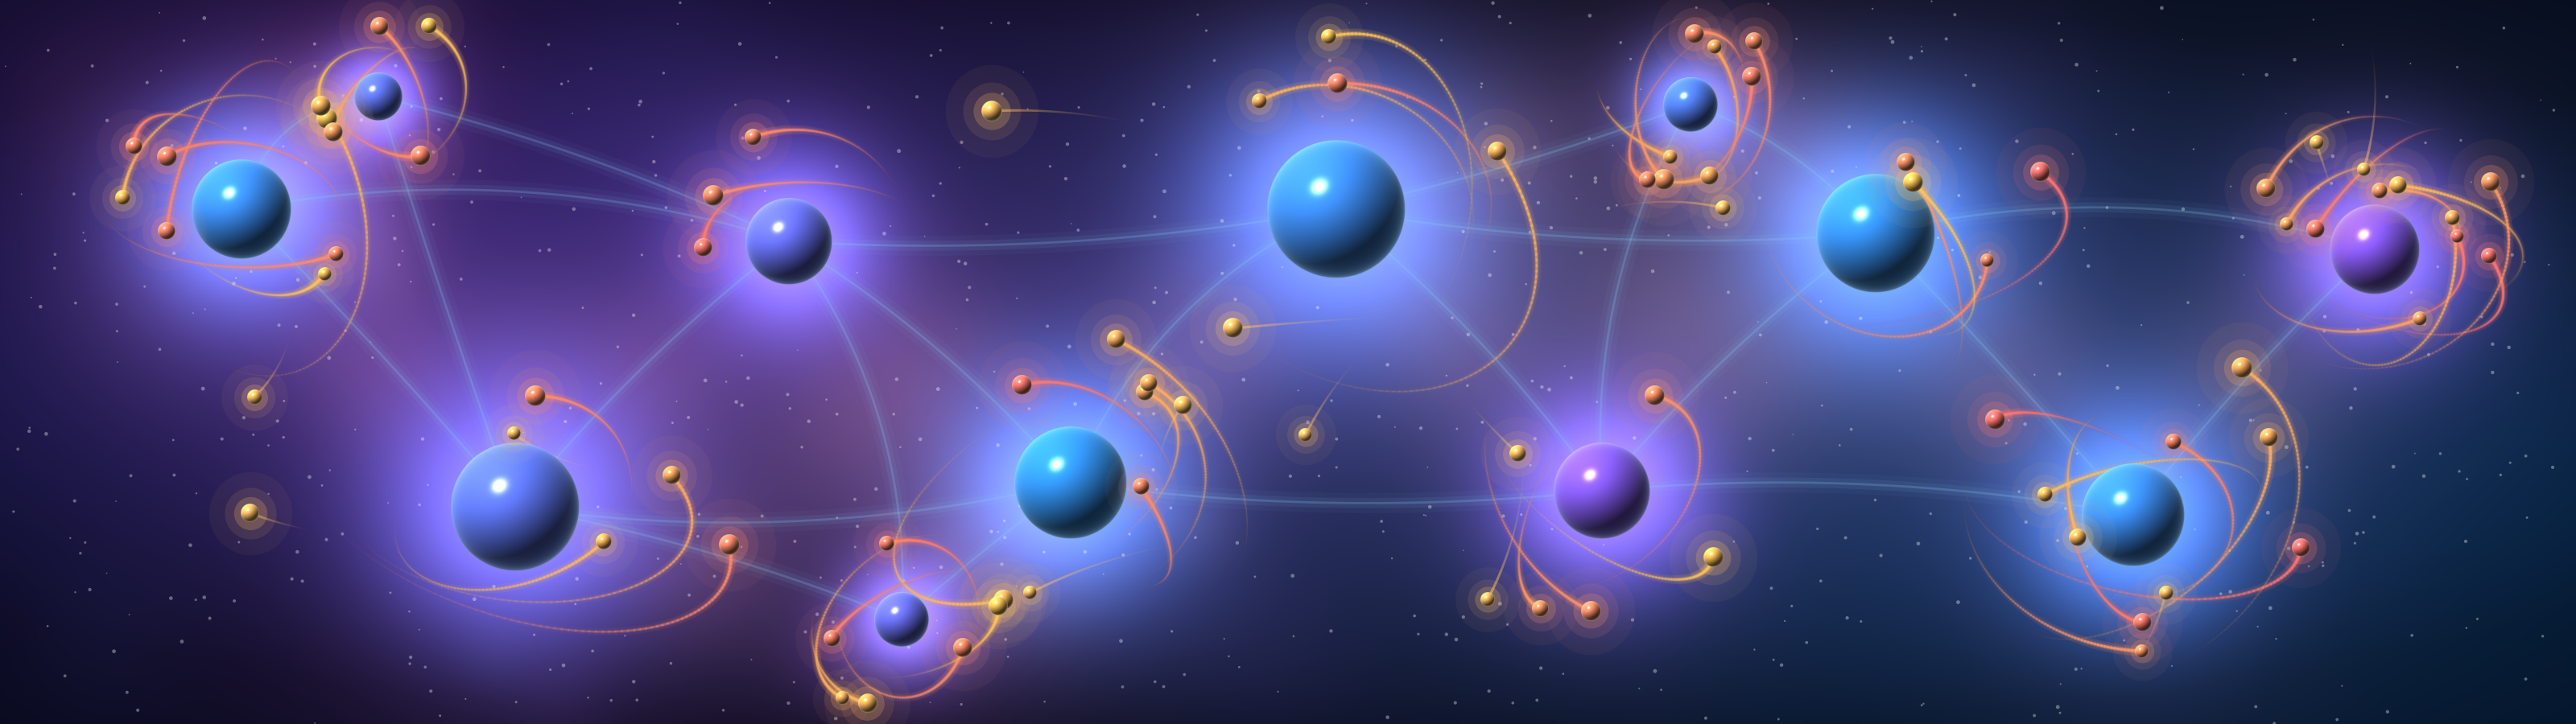
\includegraphics[width=\textwidth]{figures/many_body.png}

	\begin{columns}[T]
		\begin{column}{0.5\textwidth}
			\metroset{block=fill}
			\begin{block}<2->{First Hohenberg-Kohn Theorem}
				The ground-state density $\rho_0(\mathbf{r})$ uniquely determines the external potential,
				and therefore the full many-body wave function:
				\begin{equation*}
					|\psi_0\rangle = |\psi[\rho_0]\rangle
				\end{equation*}
				\textbf{$3N$ variables are replaced by a function of 3 variables.}
			\end{block}
		\end{column}
		\begin{column}{0.5\textwidth}
			\metroset{block=fill}
			\begin{block}<3->{Second Hohenberg-Kohn Theorem}
				The energy functional is variational: for any trial density $\rho' \neq \rho_0$,
				\[ E[\rho_0] < E[\rho'] \quad \Longleftrightarrow \quad E_0 = \min E[\rho] \]
				This gives us a practical route to the ground state.
			\end{block}
		\end{column}
	\end{columns}

\end{frame}

%-------------------------------------------------
% SLIDE 2.2 - Kohn-Sham, jellium, functionals, vdW
%-------------------------------------------------
\begin{frame}{The Kohn-Sham Scheme and the Exchange-Correlation Problem}

	\centering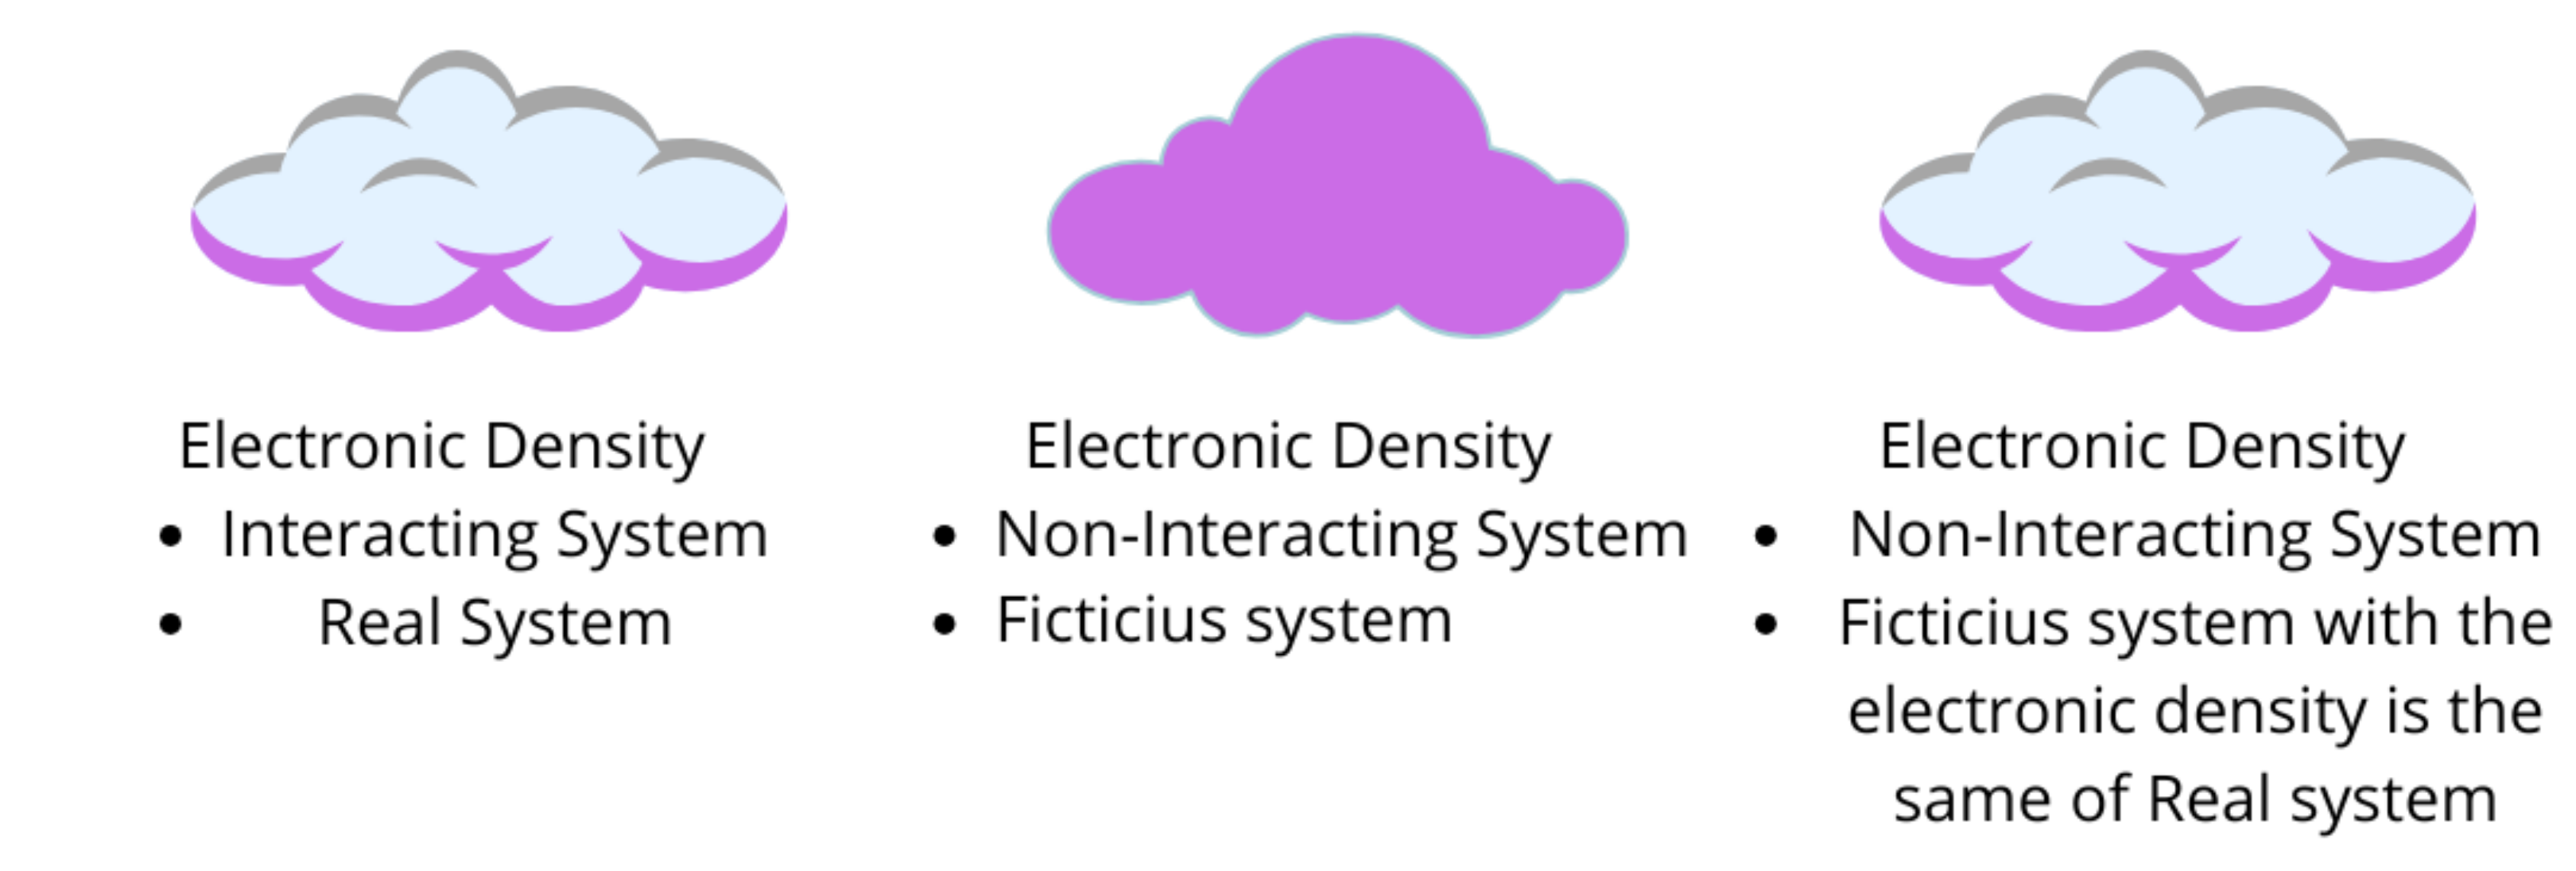
\includegraphics[height=3.5cm]{figures/kohn_sham.png}

	\vspace{0.5cm}

	\pause
	\metroset{block=fill}
	\begin{block}{Kohn-Sham mapping}
		Replace the interacting system by an \textbf{auxiliary non-interacting system}
		with the \textit{same} ground-state density:
		\begin{equation*}
			E[\rho] = T_s[\rho] + E_H[\rho] + E_{\text{xc}}[\rho]
			\qquad
			\left\{ T_s + v_H[\rho] + v_{\text{xc}}[\rho] \right\} \phi_i^{\text{KS}} = \epsilon_i \phi_i^{\text{KS}}
		\end{equation*}
		All the difficulty is now contained in a single unknown term, $E_{\text{xc}}[\rho]$.
	\end{block}

\end{frame}

%-------------------------------------------------
% SLIDE 2.2 - Kohn-Sham, jellium, functionals, vdW
%-------------------------------------------------
\begin{frame}{The Kohn-Sham Scheme and the Exchange-Correlation Problem}

	\centering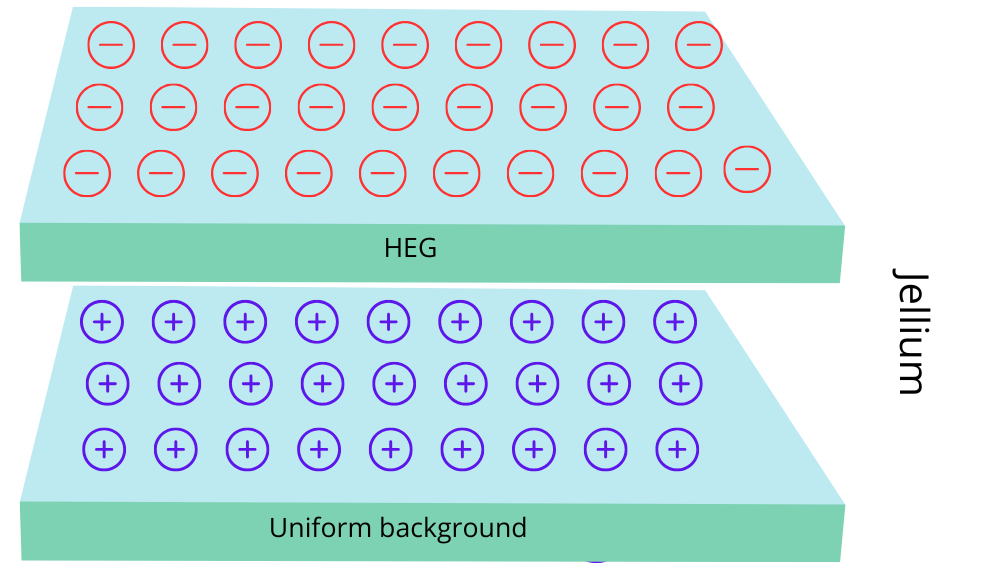
\includegraphics[height=3.5cm]{figures/HGE-jellium.png}

	\begin{columns}[T]
		\begin{column}{0.5\textwidth}
			\metroset{block=fill}
			\begin{block}<2->{From jellium to real materials}
				\begin{itemize}
					\item \textbf{LDA:} built from the homogeneous electron gas (jellium).
					\item \textbf{GGA (PBE):} adds the density gradient.
					\item \textbf{Hybrids (HSE06):} mix exact exchange, correcting the self-interaction
					      error and improving band gaps.
				\end{itemize}
			\end{block}
		\end{column}
		\begin{column}{0.5\textwidth}
			\metroset{block=fill}
			\begin{block}<3->{Long-range dispersion}
				\begin{itemize}
					\item Semilocal functionals do not describe van der Waals interactions.
					\item \textbf{Grimme-type corrections (D3)} and non-local vdW functionals are
					      essential for layered and porous systems.
				\end{itemize}
			\end{block}
		\end{column}
	\end{columns}

\end{frame}

\section{A Brief History of Atomic Basis}

\begin{frame}{Basis Sets and Numerical Atomic Orbitals}
	\metroset{block=fill}
	\begin{block}{Choosing a basis}
		Basis functions represent electronic states, and their size and flexibility
		set the balance between accuracy and computational cost.
	\end{block}

	\begin{columns}[T]
		\begin{column}{0.48\textwidth}
			\begin{block}{Plane waves}
				A widely used basis for periodic systems. Increasing the energy cutoff
				enlarges the basis and improves convergence.
			\end{block}
		\end{column}
		\begin{column}{0.48\textwidth}
			\begin{block}{Localized orbitals}
				Gaussian orbitals, numerical atomic orbitals, and wavelets can reduce
				cost and support linear-scaling methods.
			\end{block}
		\end{column}
	\end{columns}

	\begin{block}{SIESTA's numerical atomic orbitals (PAOs)}
		Generated from Kohn--Sham solutions for isolated pseudoatoms with the same
		pseudopotential and exchange-correlation functional. A confining potential
		makes them vanish beyond a cutoff radius $r_c$.
	\end{block}
	\centering
	\textbf{Single-zeta (SZ):} the minimal basis, with one radial function per occupied atomic channel.
\end{frame}

\begin{frame}{Building Flexibility: SZ, DZ, TZ, and Polarization}
	\begin{columns}[T]
		\begin{column}{0.42\textwidth}
			\begin{itemize}
				\item \textbf{SZ:} one radial function per channel.
				\item \textbf{DZ/TZ:} add radial functions to improve flexibility.
				\item \textbf{Polarization (P):} add higher-angular-momentum orbitals.
			\end{itemize}
			\metroset{block=fill}
			\begin{block}{Example: silicon}
				The illustrated basis grows from 4 orbitals (SZ) to 8 (DZ) and
				13 (DZ+P).
			\end{block}
		\end{column}
		\begin{column}{0.58\textwidth}
			\centering
			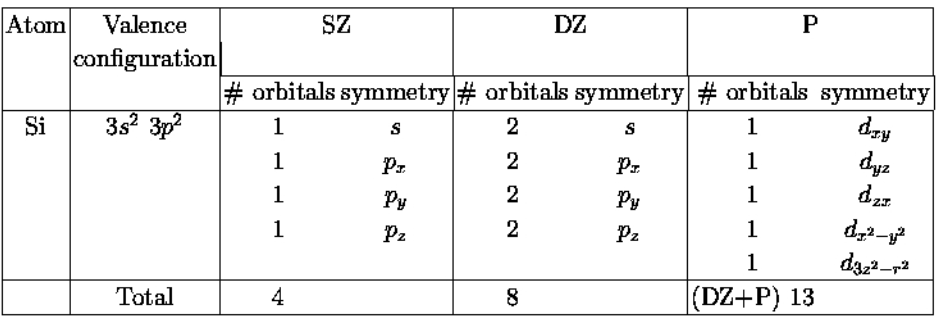
\includegraphics[width=\linewidth]{figures/basis_sz_dz_polarization.png}\\[0.2cm]
			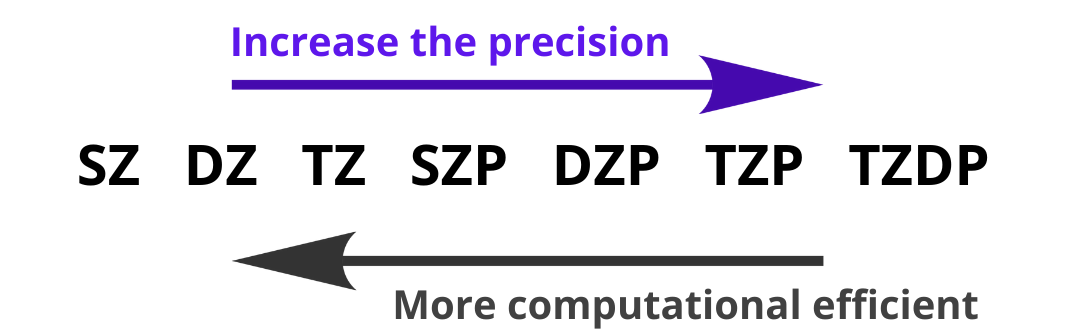
\includegraphics[width=\linewidth]{figures/basis_precision_efficiency.png}
		\end{column}
	\end{columns}
\end{frame}

\begin{frame}{Basis-Set Convergence and Cost}
	\begin{columns}[T]
		\begin{column}{0.4\textwidth}
			\metroset{block=fill}
			\begin{block}{A silicon example}
				Increasing the plane-wave cutoff lowers the energy toward
				convergence, but also increases the number of basis functions.
			\end{block}
			\begin{block}{Localized alternatives}
				SZ, DZ, TZ, and polarized NAOs offer a ladder of accuracy and
				computational cost.
			\end{block}
			{\tiny{Illustrative comparison; convergence must be checked for each system.}}
		\end{column}
		\begin{column}{0.6\textwidth}
			\metroset{block=fill}
			\centering
			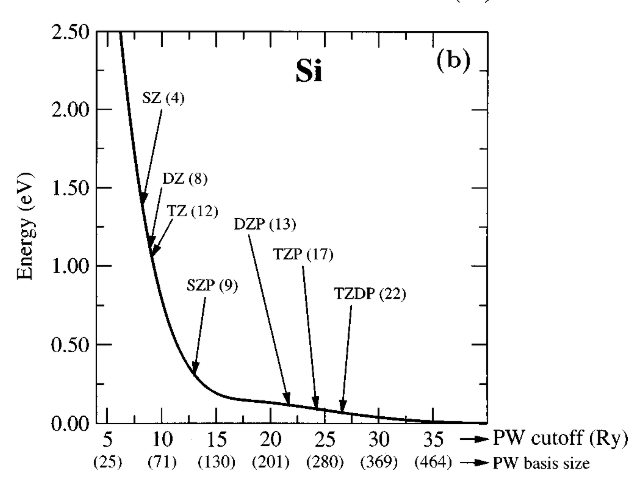
\includegraphics[height=4.9cm,keepaspectratio]{figures/basis_pw_convergence.png}
		\end{column}
	\end{columns}
\end{frame}

\begin{frame}{Cutoff Radius and \texttt{PAO.EnergyShift}}
	\begin{columns}[T]
		\begin{column}{0.42\textwidth}
			\metroset{block=fill}
			\begin{block}{Confining the orbitals}
				A confining potential truncates each PAO at a finite radius $r_c$.
				In SIESTA, \texttt{PAO.EnergyShift} sets this range through the
				orbital's energy increase under confinement.
			\end{block}
			\begin{block}{Practical trade-off}
				A larger energy shift generally produces more compact orbitals.
				Test convergence to balance locality, accuracy, and cost.
			\end{block}
		\end{column}
		\begin{column}{0.58\textwidth}
			\centering
			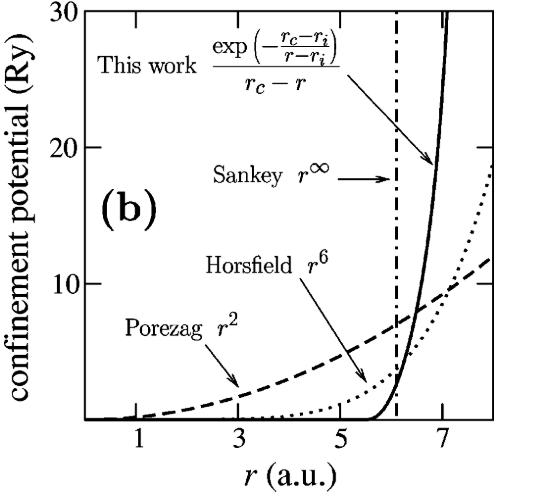
\includegraphics[height=4.8cm,keepaspectratio]{figures/pao_confinement_potential.png}\\[0.15cm]
			{\tiny{Examples of confining potentials for atomic orbitals.}}
		\end{column}
	\end{columns}
\end{frame}

\section{A Brief History of Pseudopotentials}

\begin{frame}{Why Pseudopotentials?}
	\begin{columns}[T]
		\begin{column}{0.48\textwidth}
			\metroset{block=fill}
			\begin{block}{The core-electron problem}
				Core states are tightly bound and often do not change appreciably
				in chemical processes. Treating them explicitly adds computational cost.
			\end{block}
		\end{column}
		\begin{column}{0.48\textwidth}
			\metroset{block=fill}
			\begin{block}{Plane-wave calculations}
				Rapid oscillations near nuclei require many high-frequency plane waves,
				slowing convergence.
			\end{block}
		\end{column}
	\end{columns}

	\begin{block}{The idea}
		Replace the core region by an effective potential acting on valence electrons.
		Smoother valence states need fewer plane waves while preserving the relevant
		physics outside the core.
	\end{block}
\end{frame}

\begin{frame}{From Orthogonal Plane Waves to Pseudopotentials}
	\metroset{block=fill}
	\begin{block}{A brief history}
		Herring introduced orthogonal plane waves (OPWs) in 1940; in 1959,
		Phillips--Kleinman and others developed the pseudopotential approach.
	\end{block}

	\begin{block}{Enforcing orthogonality to the core}
		An OPW removes components along the core states using the projector
		$\hat{P}_c$:
		\[
			\begin{aligned}
				|\mathbf{k}+\mathbf{G}\rangle_{\mathrm{OPW}}
				&=(1-\hat{P}_c)|\mathbf{k}+\mathbf{G}\rangle,\\
				\hat{P}_c&=\sum_c|\phi_c\rangle\langle\phi_c|.
			\end{aligned}
		\]
		This constraint can be recast as an effective repulsive contribution.
	\end{block}
\end{frame}

\begin{frame}{All-Electron vs Pseudopotential}
	\centering
	\small
	Orthogonality to core states yields a repulsive correction,
	$\hat{V}_{\mathrm{PS}}=\hat{V}+\hat{V}_{R}$; smooth pseudo-states reproduce
	valence behavior outside the core radius.

	\vspace{0.1cm}
	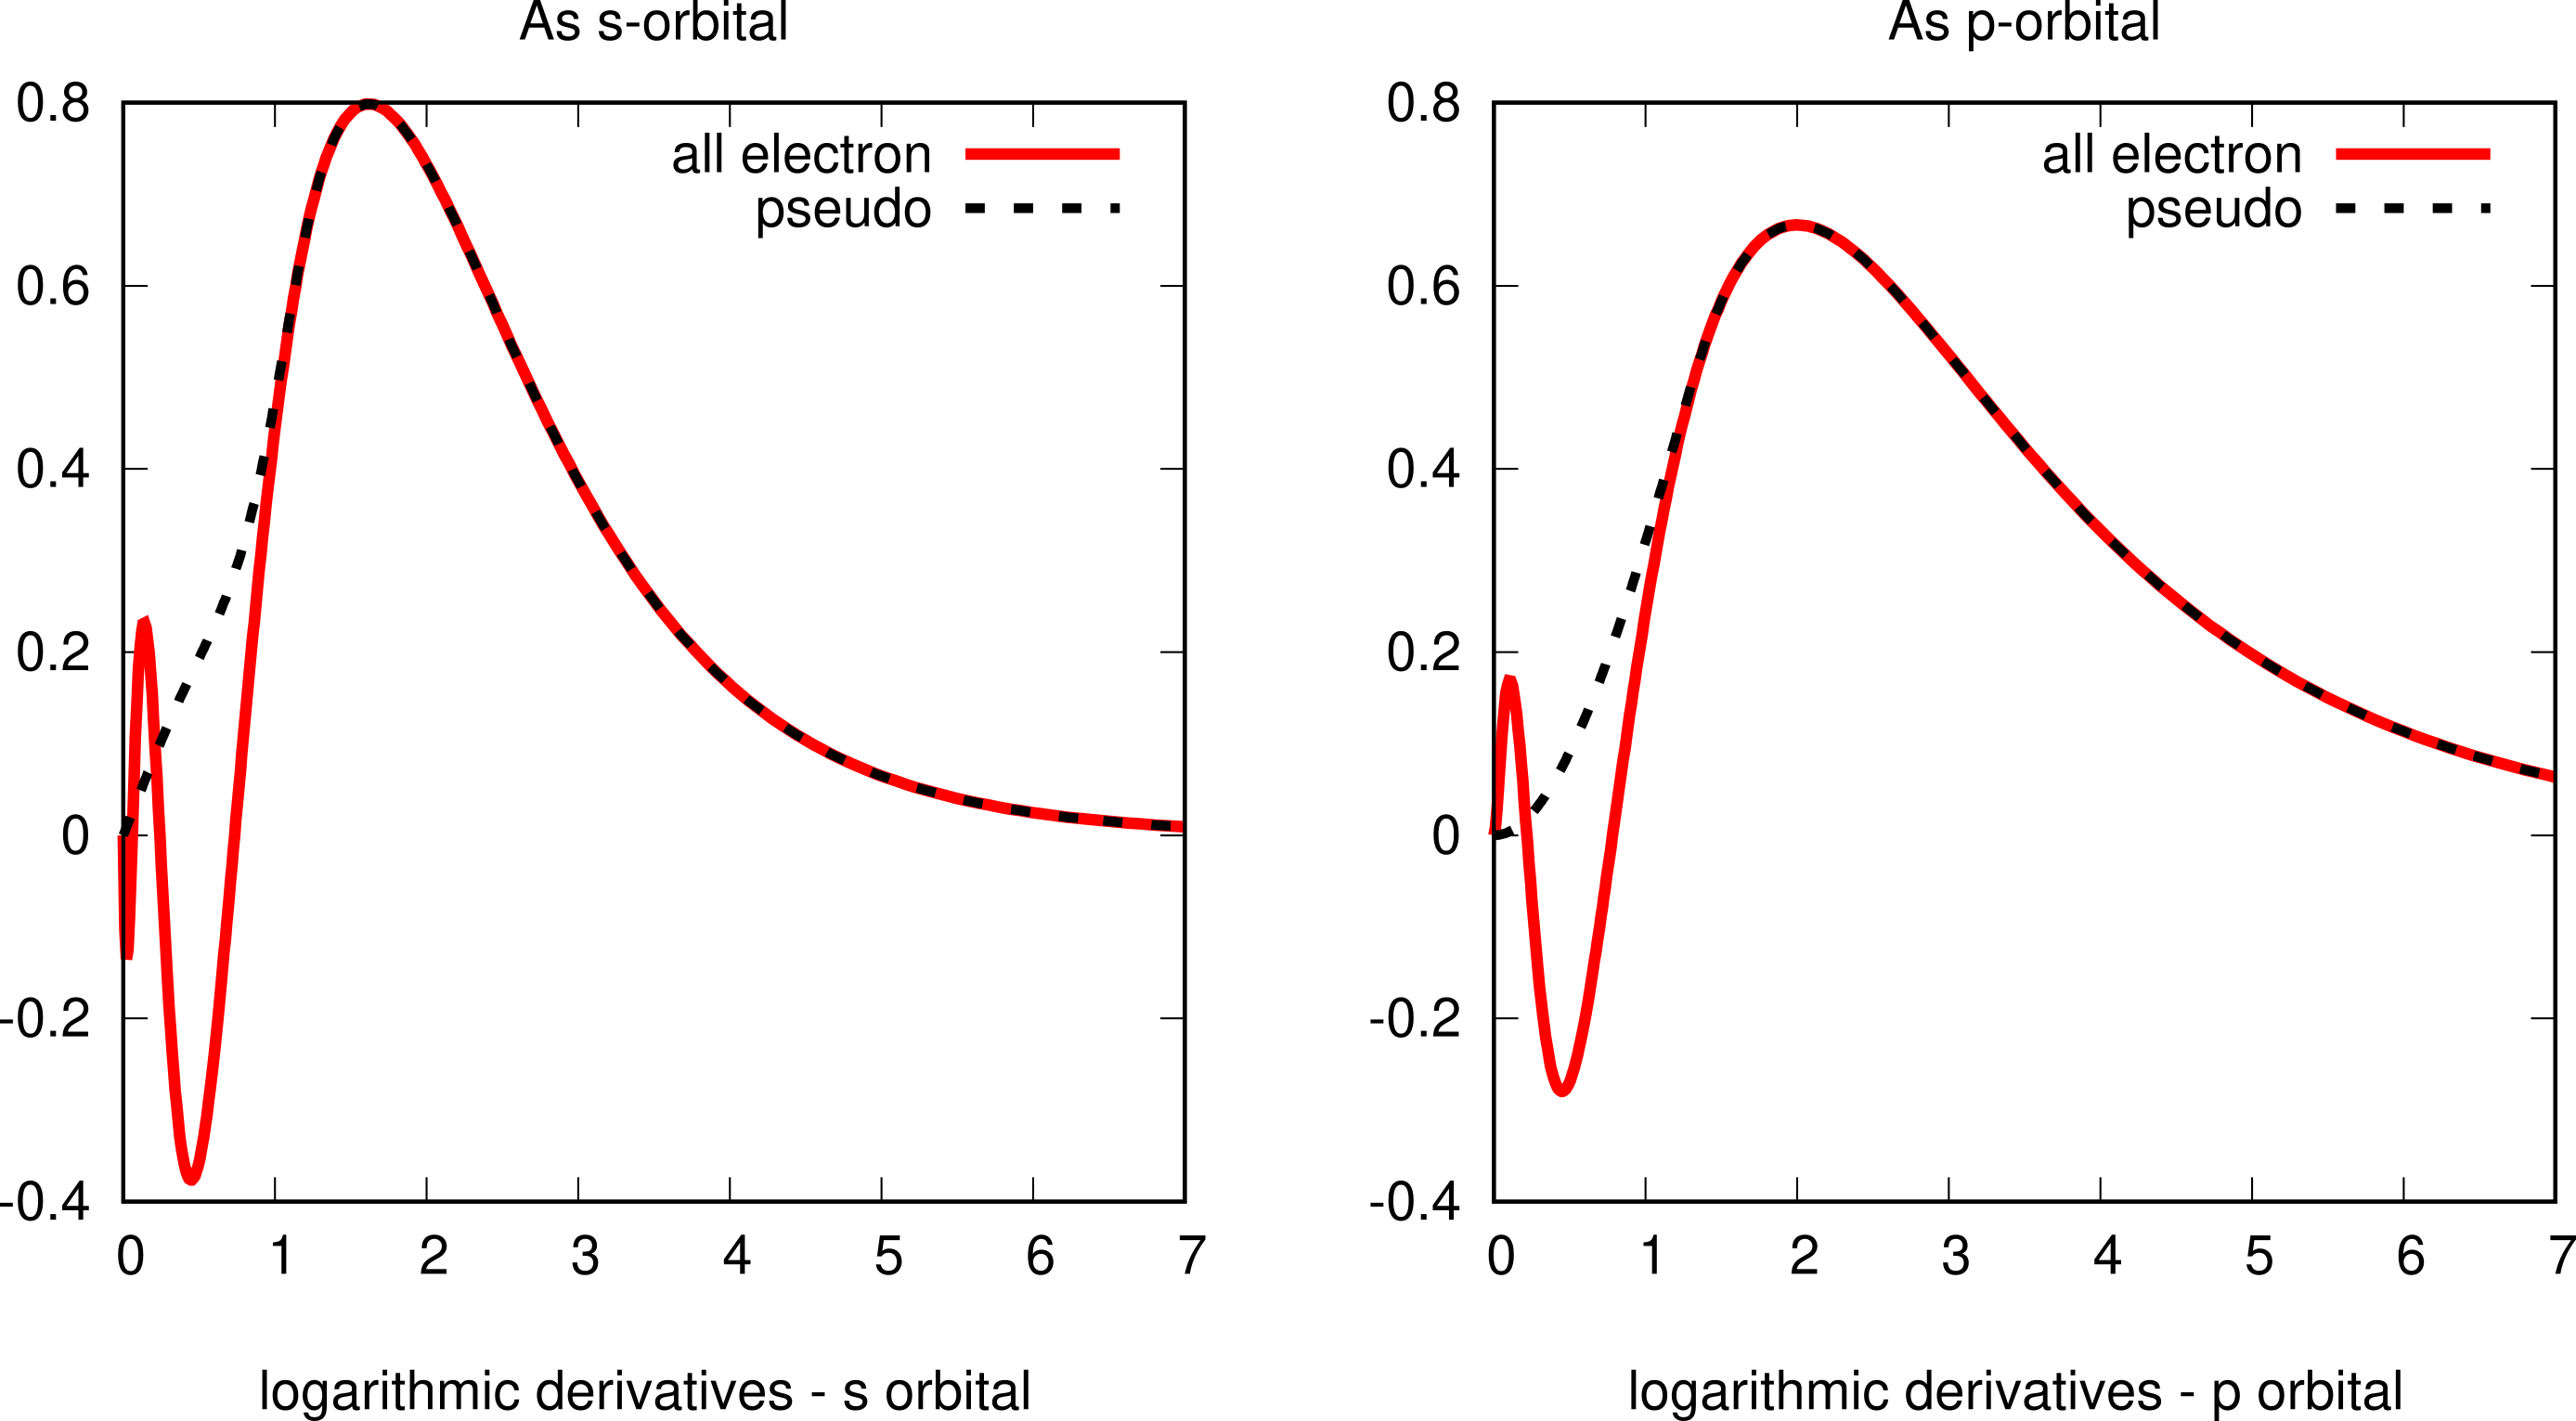
\includegraphics[width=0.88\textwidth]{figures/all_electron_vs_pseudopotential.png}
\end{frame}

%%%%%%%%%%%%%%%%%%%%%%%%%%%%%%%%%%%%%%%%%%%%%%%%%%%%%%%%
\section{Siesta Implementation}

\begin{frame}{What SIESTA Does}
	\centering
	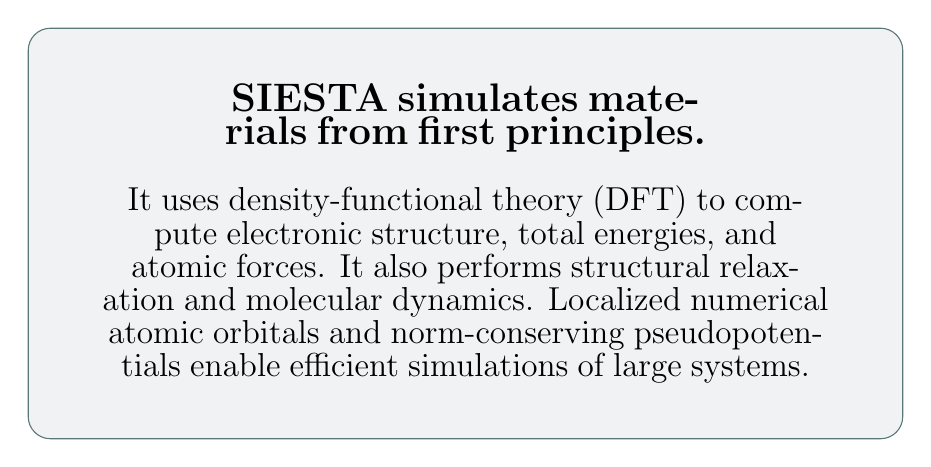
\begin{tikzpicture}[
		description/.style={
			draw=stbteal!75,fill=stbteal!7,rounded corners=8pt,
			text width=0.8\textwidth,minimum height=3.8cm,
			align=center,inner sep=20pt
		}
	]
		\node[description] {
			{\Large\bfseries SIESTA simulates materials from first principles.}\\[12pt]
			{\large It uses density-functional theory (DFT) to compute electronic
			structure, total energies, and atomic forces. It also performs
			structural relaxation and molecular dynamics. Localized numerical
			atomic orbitals and norm-conserving pseudopotentials enable efficient
			simulations of large systems.}
		};
	\end{tikzpicture}
\end{frame}

\begin{frame}{Input Files and Pseudopotentials}
	\centering
	\resizebox{0.95\textwidth}{!}{%
	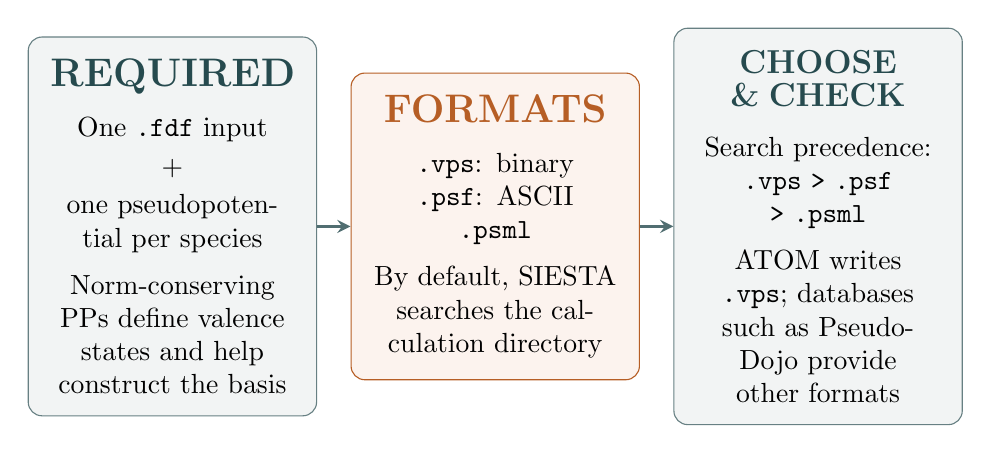
\begin{tikzpicture}[
		card/.style={
			draw=stbteal!70,fill=stbteal!6,rounded corners=5pt,
			text width=3.1cm,minimum height=2.9cm,align=center,inner sep=8pt
		},
		flow/.style={->,>=stealth,line width=1.1pt,draw=stbteal!80}
	]
		\node[card] (required) at (0,0) {
			{\color{stbteal}\Large\bfseries REQUIRED}\\[6pt]
			One \texttt{.fdf} input\\[2pt]
			+\\[2pt]
			one pseudopotential per species\\[5pt]
			Norm-conserving PPs define valence states and help construct the basis
		};
		\node[card,draw=stborange!85!black,fill=stborange!8] (formats) at (4.1,0) {
			{\color{stborange!85!black}\Large\bfseries FORMATS}\\[6pt]
			\texttt{.vps}: binary\\
			\texttt{.psf}: ASCII\\
			\texttt{.psml}\\[5pt]
			By default, SIESTA searches the calculation directory
		};
		\node[card] (source) at (8.2,0) {
			{\color{stbteal}\large\bfseries CHOOSE \& CHECK}\\[6pt]
			Search precedence:\\
			\texttt{.vps > .psf > .psml}\\[5pt]
			ATOM writes \texttt{.vps}; databases such as Pseudo-Dojo provide other formats
		};
		\draw[flow] (required.east) -- (formats.west);
		\draw[flow] (formats.east) -- (source.west);
	\end{tikzpicture}%
	}
	\vspace{0.2cm}
	\begin{alertblock}{Before production}
		Validate pseudopotential quality for the system and property of interest.
	\end{alertblock}
\end{frame}

\begin{frame}{The FDF Input: Rules That Prevent Errors}
	\centering
	\resizebox{0.96\textwidth}{!}{%
	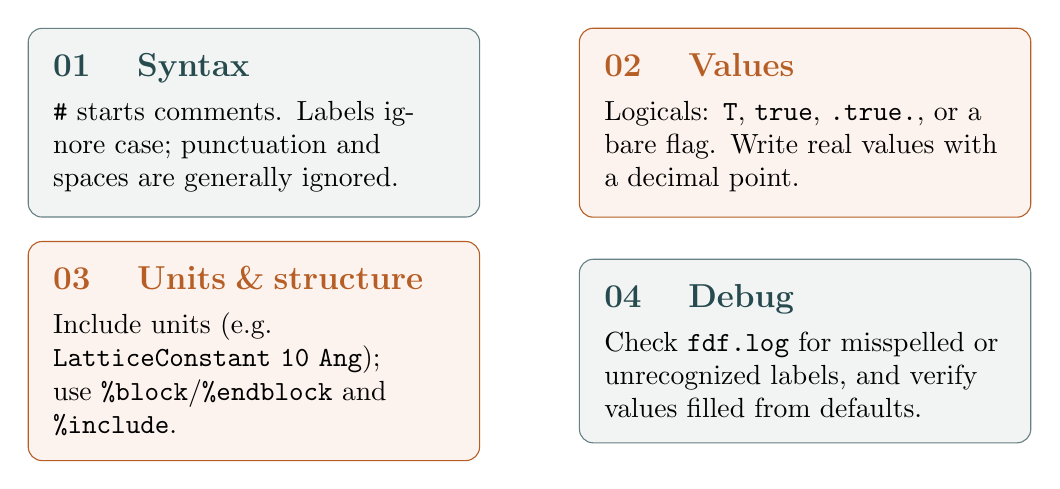
\begin{tikzpicture}[
		rule/.style={
			draw=stbteal!70,fill=stbteal!6,rounded corners=5pt,
			text width=5.1cm,minimum height=1.7cm,align=left,inner sep=9pt
		}
	]
		\node[rule] at (-3.5,1.45) {
			{\color{stbteal}\large\bfseries 01 \quad Syntax}\\[4pt]
			\texttt{\#} starts comments. Labels ignore case; punctuation and spaces are generally ignored.
		};
		\node[rule,draw=stborange!85!black,fill=stborange!8] at (3.5,1.45) {
			{\color{stborange!85!black}\large\bfseries 02 \quad Values}\\[4pt]
			Logicals: \texttt{T}, \texttt{true}, \texttt{.true.}, or a bare flag. Write real values with a decimal point.
		};
		\node[rule,draw=stborange!85!black,fill=stborange!8] at (-3.5,-1.45) {
			{\color{stborange!85!black}\large\bfseries 03 \quad Units \& structure}\\[4pt]
			Include units (e.g. \texttt{LatticeConstant 10 Ang}); use \texttt{\%block}/\texttt{\%endblock} and \texttt{\%include}.
		};
		\node[rule] at (3.5,-1.45) {
			{\color{stbteal}\large\bfseries 04 \quad Debug}\\[4pt]
			Check \texttt{fdf.log} for misspelled or unrecognized labels, and verify values filled from defaults.
		};
	\end{tikzpicture}%
	}
\end{frame}

\begin{frame}{Define the System and Its Species}
	\centering
	\resizebox{0.95\textwidth}{!}{%
	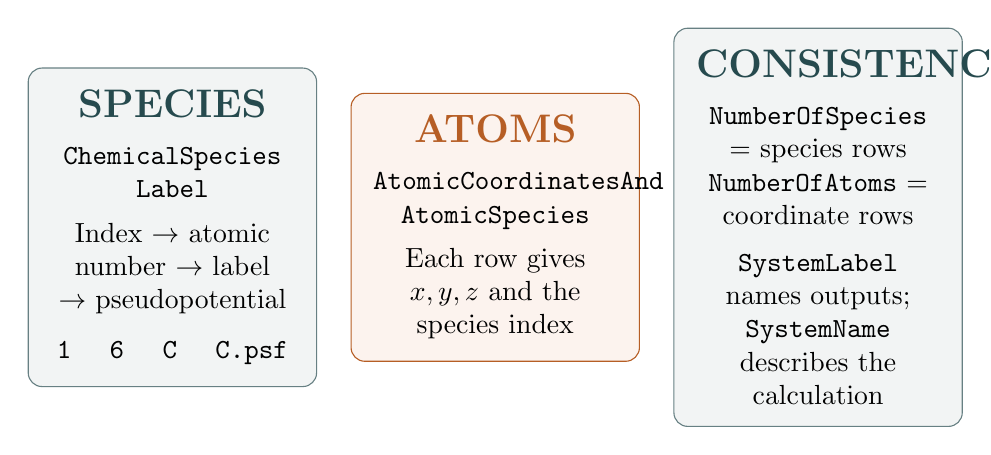
\begin{tikzpicture}[
		card/.style={
			draw=stbteal!70,fill=stbteal!6,rounded corners=5pt,
			text width=3.1cm,minimum height=3.1cm,align=center,inner sep=8pt
		}
	]
		\node[card] at (0,0) {
			{\color{stbteal}\Large\bfseries SPECIES}\\[5pt]
			\texttt{ChemicalSpecies}\\
			\texttt{Label}\\[4pt]
			Index $\rightarrow$ atomic number $\rightarrow$ label $\rightarrow$ pseudopotential\\[6pt]
			\texttt{1 \quad 6 \quad C \quad C.psf}
		};
		\node[card,draw=stborange!85!black,fill=stborange!8] at (4.1,0) {
			{\color{stborange!85!black}\Large\bfseries ATOMS}\\[5pt]
			\texttt{AtomicCoordinatesAnd}\\
			\texttt{AtomicSpecies}\\[4pt]
			Each row gives $x,y,z$ and the species index
		};
		\node[card] at (8.2,0) {
			{\color{stbteal}\Large\bfseries CONSISTENCY}\\[5pt]
			\texttt{NumberOfSpecies} = species rows\\
			\texttt{NumberOfAtoms} = coordinate rows\\[5pt]
			\texttt{SystemLabel} names outputs; \texttt{SystemName} describes the calculation
		};
	\end{tikzpicture}%
	}
\end{frame}

\begin{frame}{Choose a Basis for Accuracy and Cost}
	\centering
	\resizebox{0.95\textwidth}{!}{%
	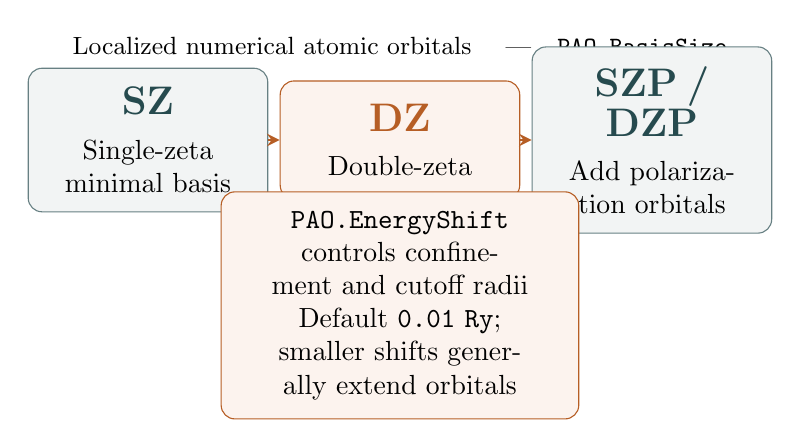
\begin{tikzpicture}[
		basis/.style={
			draw=stbteal!70,fill=stbteal!6,rounded corners=5pt,
			text width=2.55cm,minimum height=1.5cm,align=center,inner sep=7pt
		},
		control/.style={
			draw=stbteal!70,fill=stbteal!6,rounded corners=5pt,
			text width=4.05cm,minimum height=1.35cm,align=center,inner sep=7pt
		},
		flow/.style={->,>=stealth,line width=1pt,draw=stborange!85!black}
	]
		\node[font=\small] at (3.2,2.15) {
			Localized numerical atomic orbitals \quad|\quad \texttt{PAO.BasisSize}
		};
		\node[basis] (sz) at (0,0.95) {
			{\color{stbteal}\Large\bfseries SZ}\\[4pt]
			Single-zeta\\minimal basis
		};
		\node[basis,draw=stborange!85!black,fill=stborange!8] (dz) at (3.2,0.95) {
			{\color{stborange!85!black}\Large\bfseries DZ}\\[4pt]
			Double-zeta
		};
		\node[basis] (pol) at (6.4,0.95) {
			{\color{stbteal}\Large\bfseries SZP / DZP}\\[4pt]
			Add polarization orbitals
		};
		\draw[flow] (sz.east) -- (dz.west);
		\draw[flow] (dz.east) -- (pol.west);
		\node[control,draw=stborange!85!black,fill=stborange!8] at (3.2,-1.15) {
			\texttt{PAO.EnergyShift} controls confinement and cutoff radii\\
			Default \texttt{0.01 Ry}; smaller shifts generally extend orbitals
		};
	\end{tikzpicture}%
	}
\end{frame}

\begin{frame}{Converge the Electronic-Structure Calculation}
	\centering
	\resizebox{0.96\textwidth}{!}{%
	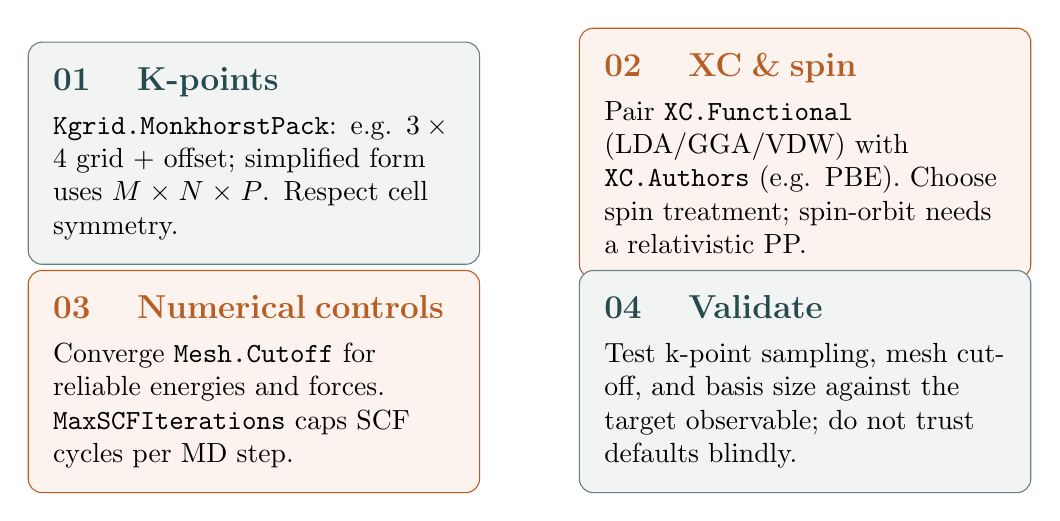
\begin{tikzpicture}[
		control/.style={
			draw=stbteal!70,fill=stbteal!6,rounded corners=5pt,
			text width=5.1cm,minimum height=1.75cm,align=left,inner sep=9pt
		}
	]
		\node[control] at (-3.5,1.45) {
			{\color{stbteal}\large\bfseries 01 \quad K-points}\\[4pt]
			\texttt{Kgrid.MonkhorstPack}: e.g. $3\times4$ grid + offset; simplified form uses $M\times N\times P$. Respect cell symmetry.
		};
		\node[control,draw=stborange!85!black,fill=stborange!8] at (3.5,1.45) {
			{\color{stborange!85!black}\large\bfseries 02 \quad XC \& spin}\\[4pt]
			Pair \texttt{XC.Functional} (LDA/GGA/VDW) with \texttt{XC.Authors} (e.g. PBE). Choose spin treatment; spin-orbit needs a relativistic PP.
		};
		\node[control,draw=stborange!85!black,fill=stborange!8] at (-3.5,-1.45) {
			{\color{stborange!85!black}\large\bfseries 03 \quad Numerical controls}\\[4pt]
			Converge \texttt{Mesh.Cutoff} for reliable energies and forces. \texttt{MaxSCFIterations} caps SCF cycles per MD step.
		};
		\node[control] at (3.5,-1.45) {
			{\color{stbteal}\large\bfseries 04 \quad Validate}\\[4pt]
			Test k-point sampling, mesh cutoff, and basis size against the target observable; do not trust defaults blindly.
		};
	\end{tikzpicture}%
	}
\end{frame}

\begin{frame}{SIESTA Output Files}
	\centering
	\resizebox{0.95\textwidth}{!}{%
	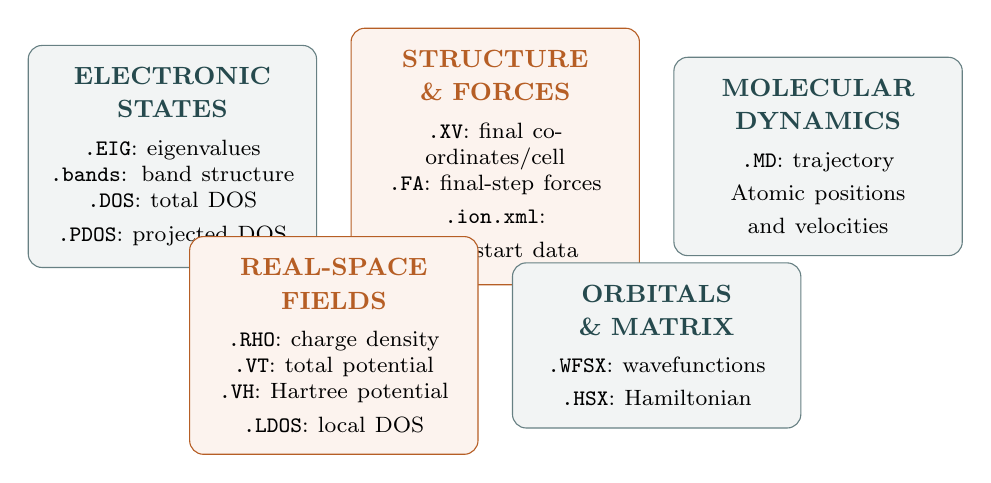
\begin{tikzpicture}[
		category/.style={
			draw=stbteal!70,fill=stbteal!6,rounded corners=5pt,
			text width=3.1cm,minimum height=1.65cm,align=center,inner sep=8pt
		},
	]
		\node[category] at (0,1.2) {
			{\color{stbteal}\small\bfseries ELECTRONIC STATES}\\[4pt]
			\footnotesize
			\texttt{.EIG}: eigenvalues\\
			\texttt{.bands}: band structure\\
			\texttt{.DOS}: total DOS\\
			\texttt{.PDOS}: projected DOS
		};
		\node[category,draw=stborange!85!black,fill=stborange!8] at (4.1,1.2) {
			{\color{stborange!85!black}\small\bfseries STRUCTURE \& FORCES}\\[4pt]
			\footnotesize
			\texttt{.XV}: final coordinates/cell\\
			\texttt{.FA}: final-step forces\\
			\texttt{.ion.xml}: ion/restart data
		};
		\node[category] at (8.2,1.2) {
			{\color{stbteal}\small\bfseries MOLECULAR DYNAMICS}\\[4pt]
			\footnotesize
			\texttt{.MD}: trajectory\\
			Atomic positions and velocities
		};
		\node[category,draw=stborange!85!black,fill=stborange!8] at (2.05,-1.2) {
			{\color{stborange!85!black}\small\bfseries REAL-SPACE FIELDS}\\[4pt]
			\footnotesize
			\texttt{.RHO}: charge density\\
			\texttt{.VT}: total potential\\
			\texttt{.VH}: Hartree potential\\
			\texttt{.LDOS}: local DOS
		};
		\node[category] at (6.15,-1.2) {
			{\color{stbteal}\small\bfseries ORBITALS \& MATRIX}\\[4pt]
			\footnotesize
			\texttt{.WFSX}: wavefunctions\\
			\texttt{.HSX}: Hamiltonian
		};
	\end{tikzpicture}%
	}
\end{frame}

%%%%%%%%%%%%%%%%%%%%%%%%%%%%%%%%%%%%%%%%%%%%%%%%%%%%%%%%
\section{Siesta ToolBox (STB)}

\begin{frame}{STB-SUITE: A Companion to SIESTA}
	\centering
	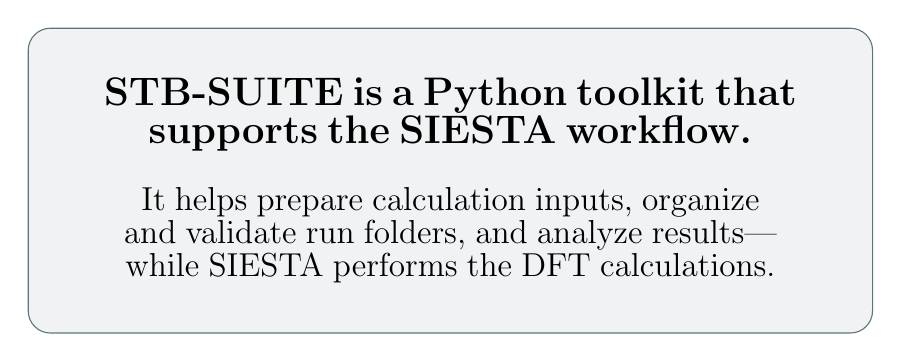
\begin{tikzpicture}[
		about/.style={
			draw=stbteal!75,
			fill=stbteal!7,
			rounded corners=8pt,
			text width=0.78\textwidth,
			minimum height=3.8cm,
			align=center,
			inner sep=18pt
		}
	]
		\node[about] {
			{\Large\bfseries STB-SUITE is a Python toolkit that supports the SIESTA workflow.}\\[12pt]
			{\large It helps prepare calculation inputs, organize and validate
			run folders, and analyze results---while SIESTA performs the DFT
			calculations.}
		};
	\end{tikzpicture}
\end{frame}

\begin{frame}{Install and Verify STB-SUITE}
	\centering
	\resizebox{0.95\textwidth}{!}{%
	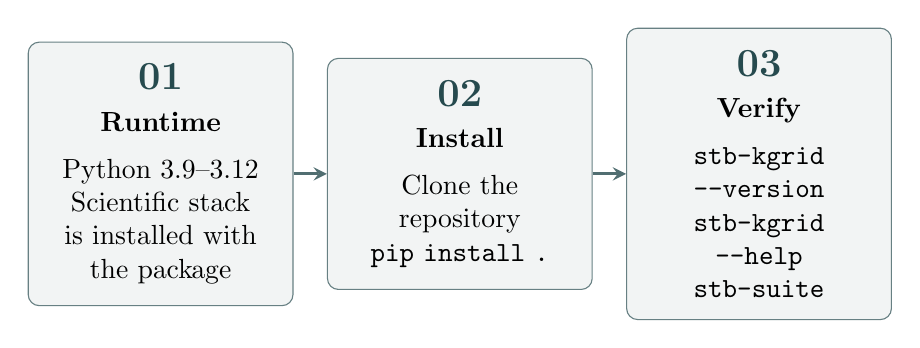
\begin{tikzpicture}[
		installstage/.style={
			draw=stbteal!70,fill=stbteal!6,rounded corners=4pt,
			text width=2.8cm,minimum height=2.55cm,align=center,inner sep=8pt
		},
		flow/.style={->,>=stealth,line width=1.1pt,draw=stbteal!80}
	]
		\node[installstage] (runtime) at (0,0) {
			{\color{stbteal}\Large\bfseries 01}\\[3pt]
			\textbf{Runtime}\\[5pt]
			Python 3.9--3.12\\
			Scientific stack is installed with the package
		};
		\node[installstage] (install) at (3.8,0) {
			{\color{stbteal}\Large\bfseries 02}\\[3pt]
			\textbf{Install}\\[5pt]
			Clone the repository\\
			\texttt{pip install .}
		};
		\node[installstage] (check) at (7.6,0) {
			{\color{stbteal}\Large\bfseries 03}\\[3pt]
			\textbf{Verify}\\[5pt]
			\texttt{stb-kgrid --version}\\
			\texttt{stb-kgrid --help}\\
			\texttt{stb-suite}
		};
		\draw[flow] (runtime.east) -- (install.west);
		\draw[flow] (install.east) -- (check.west);
	\end{tikzpicture}%
	}
	\vspace{0.35cm}
	\begin{alertblock}{Install the engines and extras you need}
		SIESTA is installed separately. MACE tools need
		\texttt{pip install ".[ml]"}; optional dependencies report how to
		install them when missing.
	\end{alertblock}
\end{frame}

\begin{frame}{A Workflow Is a Relay---Not a Black Box}
	\centering
	{\large\bfseries One relaxed structure. Many calculations. One checked property.}
	\par\vspace{0.35cm}
	\resizebox{0.97\textwidth}{!}{%
	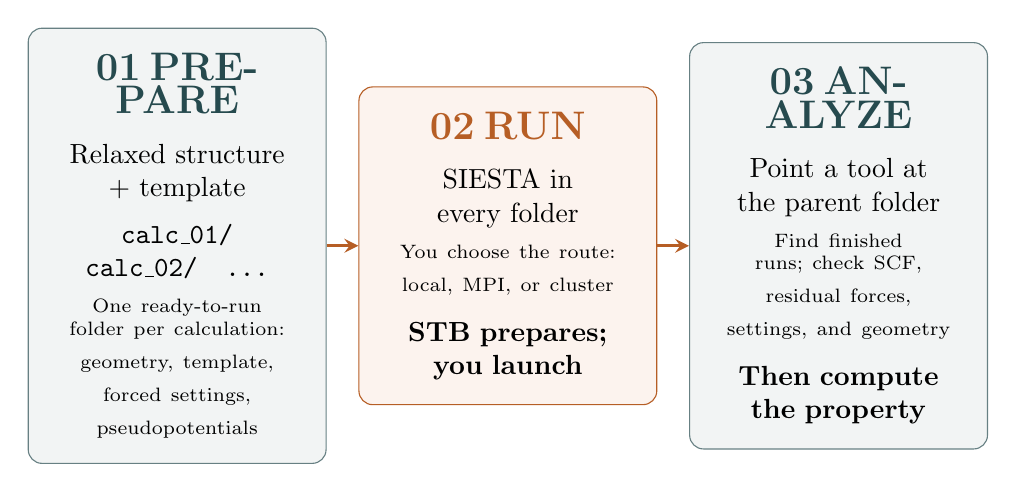
\begin{tikzpicture}[
		stage/.style={
			draw=stbteal!70,fill=stbteal!6,rounded corners=5pt,
			text width=3.15cm,minimum height=3.25cm,align=center,inner sep=9pt
		},
		run/.style={stage,draw=stborange!85!black,fill=stborange!8},
		flow/.style={->,>=stealth,line width=1.2pt,draw=stborange!85!black}
	]
		\node[stage] (prepare) at (0,0) {
			{\color{stbteal}\Large\bfseries 01 PREPARE}\\[6pt]
			Relaxed structure\\+ template\\[5pt]
			\texttt{calc\_01/}\quad\texttt{calc\_02/}\quad\texttt{...}\\[5pt]
			{\scriptsize One ready-to-run folder per calculation:\\
			geometry, template, forced settings, pseudopotentials}
		};
		\node[run] (run) at (4.2,0) {
			{\color{stborange!85!black}\Large\bfseries 02 RUN}\\[6pt]
			SIESTA in every folder\\[5pt]
			{\scriptsize You choose the route:\\
			local, MPI, or cluster}\\[6pt]
			\textbf{STB prepares; you launch}
		};
		\node[stage] (analyze) at (8.4,0) {
			{\color{stbteal}\Large\bfseries 03 ANALYZE}\\[6pt]
			Point a tool at the parent folder\\[5pt]
			{\scriptsize Find finished runs; check SCF,\\
			residual forces, settings, and geometry}\\[6pt]
			\textbf{Then compute the property}
		};
		\draw[flow] (prepare.east) -- (run.west);
		\draw[flow] (run.east) -- (analyze.west);
	\end{tikzpicture}%
	}
	\vspace{0.25cm}
	\begin{alertblock}{The handoff is the point}
		Analysis is a quality gate: unfinished or inconsistent runs are reported.
		Some methods loop back to \textbf{PREPARE} after an intermediate SIESTA run.
	\end{alertblock}
	\hfill{\scriptsize STB Manual, Chapter 5}
\end{frame}

\begin{frame}{Two Ways to Run a Tool}
	\centering
	\resizebox{0.9\textwidth}{!}{%
	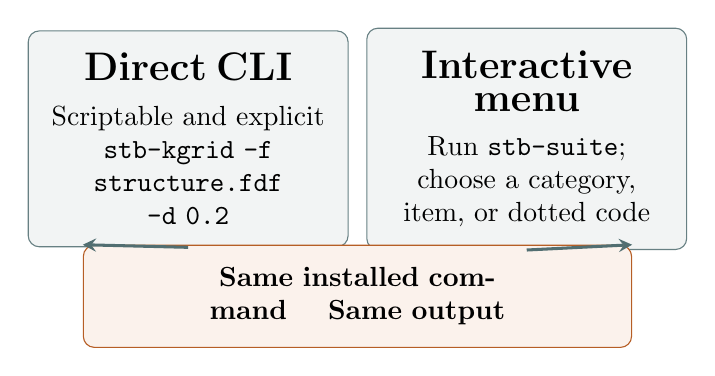
\begin{tikzpicture}[
		mode/.style={
			draw=stbteal!70,fill=stbteal!6,rounded corners=4pt,
			text width=3.5cm,minimum height=1.75cm,align=center,inner sep=8pt
		},
		common/.style={
			draw=stborange!85!black,fill=stborange!9,rounded corners=4pt,
			text width=6.4cm,minimum height=1.15cm,align=center,inner sep=8pt
		},
		flow/.style={->,>=stealth,line width=1.1pt,draw=stbteal!80}
	]
		\node[mode] (cli) at (-2.15,0) {
			{\Large\bfseries Direct CLI}\\[4pt]
			Scriptable and explicit\\
			\texttt{stb-kgrid -f structure.fdf -d 0.2}
		};
		\node[mode] (menu) at (2.15,0) {
			{\Large\bfseries Interactive menu}\\[4pt]
			Run \texttt{stb-suite}; choose a category, item, or dotted code
		};
		\node[common] (same) at (0,-2.0) {
			\textbf{Same installed command \quad Same output}
		};
		\draw[flow] (cli.south) -- (same.north west);
		\draw[flow] (menu.south) -- (same.north east);
	\end{tikzpicture}%
	}
	\vspace{0.3cm}
	\begin{alertblock}{You control the calculation}
		STB does not choose how SIESTA is scheduled or launched; the menu
		and CLI are two interfaces to the same tools.
	\end{alertblock}
\end{frame}

\begin{frame}{Reports, Diagnostics, and Citations}
	\centering
	\resizebox{0.95\textwidth}{!}{%
	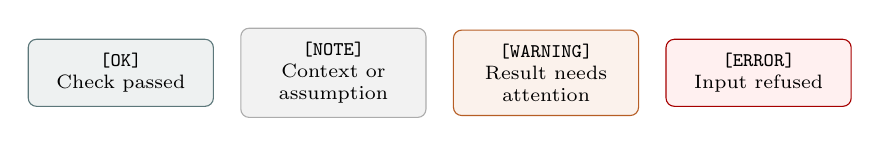
\begin{tikzpicture}[
		status/.style={
			rounded corners=3pt,text width=2cm,minimum height=0.8cm,
			align=center,inner sep=5pt,font=\scriptsize
		}
	]
		\node[status,draw=stbteal!75,fill=stbteal!8] at (0,0)
			{\textbf{\texttt{[OK]}}\\Check passed};
		\node[status,draw=gray!65,fill=gray!10] at (2.7,0)
			{\textbf{\texttt{[NOTE]}}\\Context or assumption};
		\node[status,draw=stborange!85!black,fill=stborange!9] at (5.4,0)
			{\textbf{\texttt{[WARNING]}}\\Result needs attention};
		\node[status,draw=red!65!black,fill=red!6] at (8.1,0)
			{\textbf{\texttt{[ERROR]}}\\Input refused};
	\end{tikzpicture}%
	}
	\vspace{0.35cm}
	\begin{columns}[T]
		\begin{column}{0.48\textwidth}
			\metroset{block=fill}
			\begin{block}{Read the full report}
				Numbered sections cover metadata, checks, results, and
				warnings. \texttt{--save-report} writes a copy; other
				markers include \texttt{[SKIPPED]}, \texttt{[UNVERIFIED]},
				and \texttt{[EXTRAPOLATED]}.
			\end{block}
		\end{column}
		\begin{column}{0.48\textwidth}
			\metroset{block=fill}
			\begin{block}{Keep data and provenance}
				Tools merge citable sources into \texttt{references.bib}.
				Plots may save \texttt{.dat}+\texttt{.gplot}; trajectories
				support XSF, PDB, or extended XYZ.
			\end{block}
		\end{column}
	\end{columns}
\end{frame}

\begin{frame}{Separate Geometry from Calculation Settings}
	\centering
	\resizebox{0.9\textwidth}{!}{%
	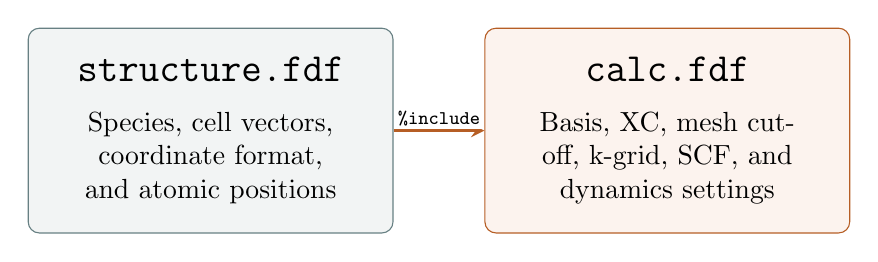
\begin{tikzpicture}[
		file/.style={
			draw=stbteal!70,fill=stbteal!6,rounded corners=4pt,
			text width=4cm,minimum height=2.6cm,align=center,inner sep=9pt
		},
		flow/.style={->,>=stealth,line width=1.1pt,draw=stborange!85!black}
	]
		\node[file] (structure) at (0,0) {
			{\Large\bfseries\texttt{structure.fdf}}\\[6pt]
			Species, cell vectors, coordinate format, and atomic positions
		};
		\node[file,draw=stborange!85!black,fill=stborange!8] (calc) at (5.8,0) {
			{\Large\bfseries\texttt{calc.fdf}}\\[6pt]
			Basis, XC, mesh cutoff, k-grid, SCF, and dynamics settings
		};
		\draw[flow] (structure.east) -- node[above,font=\scriptsize,fill=white,inner sep=1pt]
			{\texttt{\%include}} (calc.west);
	\end{tikzpicture}%
	}
	\vspace{0.35cm}
	\begin{alertblock}{Why keep them separate?}
		STB can prepare many geometries while copying your calculation
		template unchanged, so the intended level of theory stays explicit.
		A self-contained FDF is also supported by several tools.
	\end{alertblock}
\end{frame}

\begin{frame}{Override Settings Without Editing Templates}
	\centering
	\resizebox{0.95\textwidth}{!}{%
	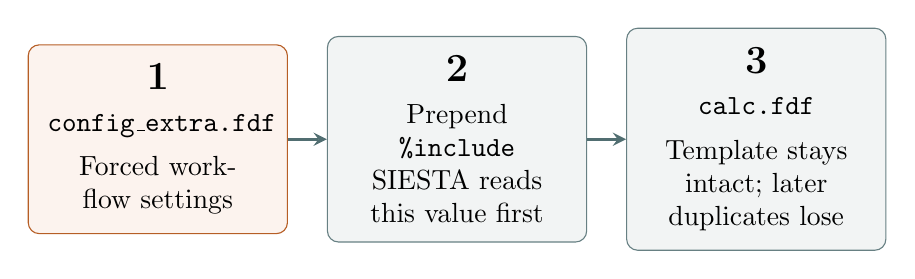
\begin{tikzpicture}[
		overridebox/.style={
			draw=stbteal!70,fill=stbteal!6,rounded corners=4pt,
			text width=2.8cm,minimum height=2.3cm,align=center,inner sep=7pt
		},
		flow/.style={->,>=stealth,line width=1.1pt,draw=stbteal!80}
	]
		\node[overridebox,draw=stborange!85!black,fill=stborange!8] (sidecar) at (0,0) {
			{\Large\bfseries 1}\\[3pt]
			\texttt{config\_extra.fdf}\\[4pt]
			Forced workflow settings
		};
		\node[overridebox] (first) at (3.8,0) {
			{\Large\bfseries 2}\\[3pt]
			Prepend \texttt{\%include}\\
			SIESTA reads this value first
		};
		\node[overridebox] (template) at (7.6,0) {
			{\Large\bfseries 3}\\[3pt]
			\texttt{calc.fdf}\\[4pt]
			Template stays intact; later duplicates lose
		};
		\draw[flow] (sidecar.east) -- (first.west);
		\draw[flow] (first.east) -- (template.west);
	\end{tikzpicture}%
	}
	\vspace{0.3cm}
	\metroset{block=fill}
	\begin{block}{Why order matters}
		FDF labels ignore case and punctuation; the first occurrence wins.
		An include appended later cannot override an existing template value.
	\end{block}
	\begin{alertblock}{Practical rule}
		Prepend the sidecar so forced settings take precedence without
		editing the user's calculation template.
	\end{alertblock}
\end{frame}

\begin{frame}{Pseudopotentials: Sources and Validation}
	\centering
	\resizebox{0.95\textwidth}{!}{%
	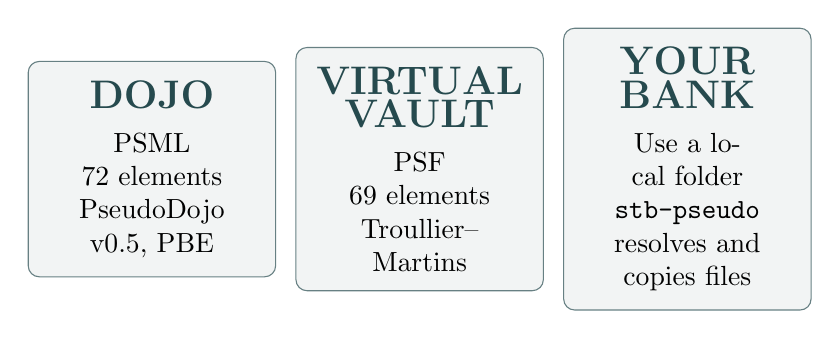
\begin{tikzpicture}[
		source/.style={
			draw=stbteal!70,fill=stbteal!6,rounded corners=4pt,
			text width=2.65cm,minimum height=2.25cm,align=center,inner sep=7pt
		}
	]
		\node[source] at (0,0) {
			{\color{stbteal}\Large\bfseries DOJO}\\[4pt]
			PSML\\
			72 elements\\
			PseudoDojo v0.5, PBE
		};
		\node[source] at (3.4,0) {
			{\color{stbteal}\Large\bfseries VIRTUAL VAULT}\\[4pt]
			PSF\\
			69 elements\\
			Troullier--Martins
		};
		\node[source] at (6.8,0) {
			{\color{stbteal}\Large\bfseries YOUR BANK}\\[4pt]
			Use a local folder\\
			\texttt{stb-pseudo} resolves and copies files
		};
	\end{tikzpicture}%
	}
	\vspace{0.3cm}
	\begin{block}{Portable calculation folders}
		STB copies pseudopotentials instead of symlinking them, so folders
		remain usable when moved or archived.
	\end{block}
	\begin{alertblock}{A database is not a quality guarantee}
		Validate a new pseudopotential against a known property for your
		system before production calculations.
	\end{alertblock}
\end{frame}

\begin{frame}{Vacuum, Dimensionality, and Boundaries}
	\centering
	\resizebox{0.94\textwidth}{!}{%
	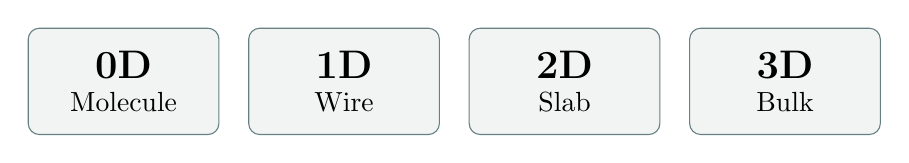
\begin{tikzpicture}[
		dimension/.style={
			draw=stbteal!70,fill=stbteal!6,rounded corners=4pt,
			text width=2cm,minimum height=1.35cm,align=center,inner sep=6pt
		}
	]
		\node[dimension] at (0,0)
			{{\Large\bfseries 0D}\\Molecule};
		\node[dimension] at (2.8,0)
			{{\Large\bfseries 1D}\\Wire};
		\node[dimension] at (5.6,0)
			{{\Large\bfseries 2D}\\Slab};
		\node[dimension] at (8.4,0)
			{{\Large\bfseries 3D}\\Bulk};
	\end{tikzpicture}%
	}
	\vspace{0.25cm}
	\metroset{block=fill}
	\begin{block}{How the dimensionality is found}
		A wrap-aware largest-gap test identifies vacuum axes
		(\texttt{--vacuum-gap}, default 10 \AA); this affects k-grids and
		which properties or strains are meaningful.
	\end{block}
	\begin{alertblock}{Respect periodic boundaries}
		Coordinates are wrapped and distances use the minimum-image
		convention. Cell strains require fractional coordinates; Cartesian
		inputs are refused.
	\end{alertblock}
\end{frame}

\begin{frame}{SIESTA Files Read by STB}
	\centering
	\resizebox{0.95\textwidth}{!}{%
	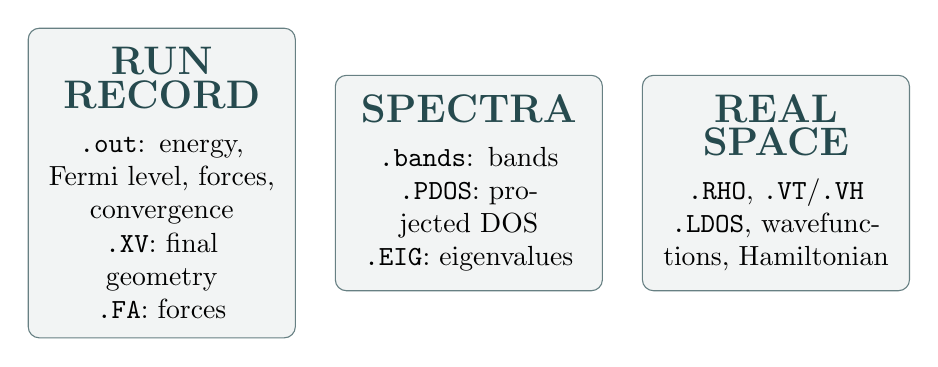
\begin{tikzpicture}[
		files/.style={
			draw=stbteal!70,fill=stbteal!6,rounded corners=4pt,
			text width=2.9cm,minimum height=2.35cm,align=center,inner sep=7pt
		}
	]
		\node[files] at (0,0) {
			{\color{stbteal}\Large\bfseries RUN RECORD}\\[4pt]
			\texttt{.out}: energy, Fermi level, forces, convergence\\
			\texttt{.XV}: final geometry\\
			\texttt{.FA}: forces
		};
		\node[files] at (3.9,0) {
			{\color{stbteal}\Large\bfseries SPECTRA}\\[4pt]
			\texttt{.bands}: bands\\
			\texttt{.PDOS}: projected DOS\\
			\texttt{.EIG}: eigenvalues
		};
		\node[files] at (7.8,0) {
			{\color{stbteal}\Large\bfseries REAL SPACE}\\[4pt]
			\texttt{.RHO}, \texttt{.VT}/\texttt{.VH}\\
			\texttt{.LDOS}, wavefunctions, Hamiltonian
		};
	\end{tikzpicture}%
	}
	\vspace{0.3cm}
	\begin{alertblock}{Match the file to the analysis}
		Some data require explicit SIESTA flags (for example
		\texttt{SaveRho}). STB can locate \texttt{calc.out} or accept an
		explicit path; filenames need not match \texttt{SystemLabel}.
	\end{alertblock}
\end{frame}

\begin{frame}{The Prepare--Run--Analyze Cycle}
	\centering
	\resizebox{0.96\textwidth}{!}{%
	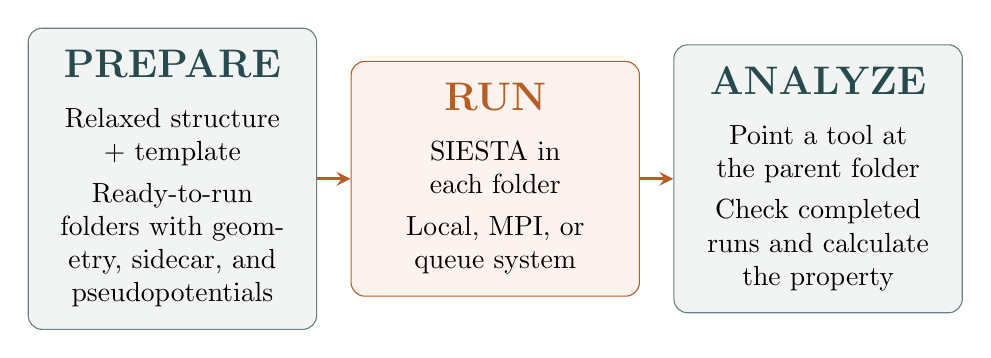
\begin{tikzpicture}[
		stage/.style={
			draw=stbteal!70,fill=stbteal!6,rounded corners=5pt,
			text width=3.1cm,minimum height=2.7cm,align=center,inner sep=8pt
		},
		flow/.style={->,>=stealth,line width=1.2pt,draw=stborange!85!black}
	]
		\node[stage] (prepare) at (0,0) {
			{\color{stbteal}\Large\bfseries PREPARE}\\[6pt]
			Relaxed structure + template\\[3pt]
			Ready-to-run folders with geometry, sidecar, and pseudopotentials
		};
		\node[stage,draw=stborange!85!black,fill=stborange!8] (run) at (4.1,0) {
			{\color{stborange!85!black}\Large\bfseries RUN}\\[6pt]
			SIESTA in each folder\\[3pt]
			Local, MPI, or queue system
		};
		\node[stage] (analyze) at (8.2,0) {
			{\color{stbteal}\Large\bfseries ANALYZE}\\[6pt]
			Point a tool at the parent folder\\[3pt]
			Check completed runs and calculate the property
		};
		\draw[flow] (prepare.east) -- (run.west);
		\draw[flow] (run.east) -- (analyze.west);
	\end{tikzpicture}%
	}
	\vspace{0.35cm}
	\begin{alertblock}{Some workflows need intermediate stages}
		Additional preparation may depend on results from an earlier SIESTA
		run; the same staged pattern still applies.
	\end{alertblock}
\end{frame}

\begin{frame}{STB-SUITE Sections}
	\centering
	\resizebox{0.95\textwidth}{!}{%
	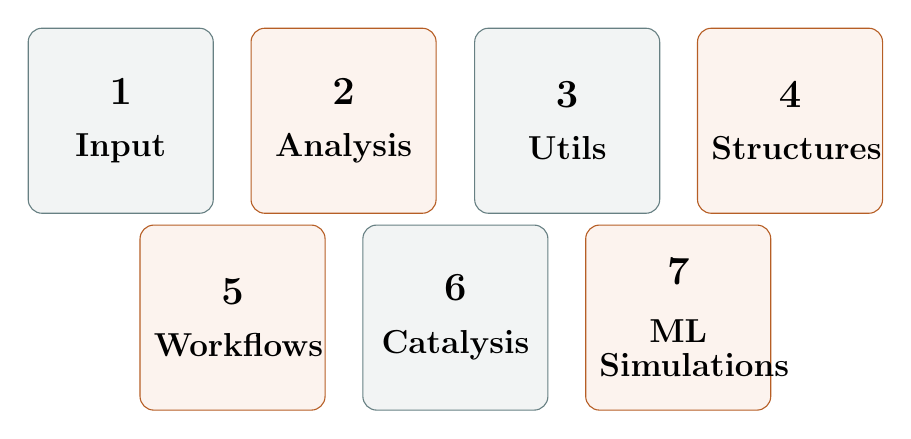
\begin{tikzpicture}[
		section/.style={
			draw=stbteal!70,fill=stbteal!6,rounded corners=5pt,
			minimum width=2.35cm,minimum height=2.35cm,
			text width=2cm,align=center,inner sep=4pt
		},
		sectionalt/.style={
			section,draw=stborange!85!black,fill=stborange!8
		}
	]
		\node[section] at (-4.25,1.25) {
			{\Large\bfseries 1}\\[7pt]
			{\large\bfseries Input}
		};
		\node[sectionalt] at (-1.42,1.25) {
			{\Large\bfseries 2}\\[7pt]
			{\large\bfseries Analysis}
		};
		\node[section] at (1.42,1.25) {
			{\Large\bfseries 3}\\[7pt]
			{\large\bfseries Utils}
		};
		\node[sectionalt] at (4.25,1.25) {
			{\Large\bfseries 4}\\[7pt]
			{\large\bfseries Structures}
		};
		\node[sectionalt] at (-2.83,-1.25) {
			{\Large\bfseries 5}\\[7pt]
			{\large\bfseries Workflows}
		};
		\node[section] at (0,-1.25) {
			{\Large\bfseries 6}\\[7pt]
			{\large\bfseries Catalysis}
		};
		\node[sectionalt] at (2.83,-1.25) {
			{\Large\bfseries 7}\\[7pt]
			{\large\bfseries ML\\Simulations}
		};
	\end{tikzpicture}%
	}
\end{frame}

%%%%%%%%%%%%%%%%%%%%%%%%%%%%%%%%%%%%%%%%%%%%%%%%%%%%%%%%
\section{Practical Part}

\begin{frame}{Practical Structures: GaAs and hBN}
	\begin{columns}[T]
		\begin{column}{0.49\textwidth}
			\metroset{block=fill}
			\begin{block}{Zincblende GaAs}
				\centering
				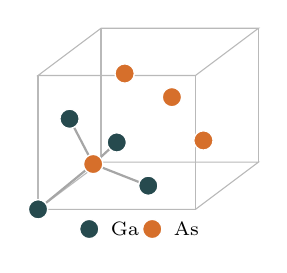
\begin{tikzpicture}[
					bond/.style={draw=gray!70,line width=0.8pt},
					ga/.style={circle,fill=stbteal,draw=white,line width=0.5pt,minimum size=7pt,inner sep=0pt},
					asatom/.style={circle,fill=stborange,draw=white,line width=0.5pt,minimum size=7pt,inner sep=0pt}
				]
					\draw[gray!55] (0,0)--(2,0)--(2.8,0.6)--(0.8,0.6)--cycle;
					\draw[gray!55] (0,1.7)--(2,1.7)--(2.8,2.3)--(0.8,2.3)--cycle;
					\draw[gray!55] (0,0)--(0,1.7);
					\draw[gray!55] (2,0)--(2,1.7);
					\draw[gray!55] (0.8,0.6)--(0.8,2.3);
					\draw[gray!55] (2.8,0.6)--(2.8,2.3);
					\draw[bond] (0.7,0.575)--(0,0);
					\draw[bond] (0.7,0.575)--(0.4,1.15);
					\draw[bond] (0.7,0.575)--(1,0.85);
					\draw[bond] (0.7,0.575)--(1.4,0.3);
					\node[ga] at (0,0) {};
					\node[ga] at (0.4,1.15) {};
					\node[ga] at (1,0.85) {};
					\node[ga] at (1.4,0.3) {};
					\node[asatom] at (0.7,0.575) {};
					\node[asatom] at (1.1,1.725) {};
					\node[asatom] at (1.7,1.425) {};
					\node[asatom] at (2.1,0.875) {};
					\node[ga] at (0.65,-0.25) {};
					\node[anchor=west,font=\scriptsize] at (0.8,-0.25) {Ga};
					\node[asatom] at (1.45,-0.25) {};
					\node[anchor=west,font=\scriptsize] at (1.6,-0.25) {As};
				\end{tikzpicture}

				\scriptsize Cubic 3D lattice: interpenetrating fcc sublattices;
				each atom has four nearest neighbors of the other species.
			\end{block}
		\end{column}
		\begin{column}{0.49\textwidth}
			\metroset{block=fill}
			\begin{block}{Hexagonal Boron Nitride (hBN)}
				\centering
				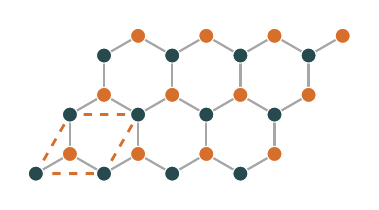
\begin{tikzpicture}[
					bond/.style={draw=gray!70,line width=0.8pt},
					boron/.style={circle,fill=stbteal,draw=white,line width=0.4pt,minimum size=5.5pt,inner sep=0pt},
					nitrogen/.style={circle,fill=stborange,draw=white,line width=0.4pt,minimum size=5.5pt,inner sep=0pt}
				]
					\foreach \i in {0,1,2,3} {
						\foreach \j in {0,1,2} {
							\coordinate (A\i\j) at ({0.866*\i+0.433*\j},{0.75*\j});
							\coordinate (B\i\j) at ({0.866*\i+0.433*\j+0.433},{0.75*\j+0.25});
						}
					}
					\foreach \i in {0,1,2,3} {
						\foreach \j in {0,1,2} {
							\draw[bond] (A\i\j)--(B\i\j);
						}
					}
					\foreach \i/\ip in {0/1,1/2,2/3} {
						\foreach \j in {0,1,2} {
							\draw[bond] (B\i\j)--(A\ip\j);
						}
					}
					\foreach \i in {0,1,2,3} {
						\draw[bond] (B\i0)--(A\i1);
						\draw[bond] (B\i1)--(A\i2);
					}
					\draw[draw=stborange,dashed,line width=1pt]
						(A00)--(A10)--(A11)--(A01)--cycle;
					\foreach \i in {0,1,2,3} {
						\foreach \j in {0,1,2} {
							\node[boron] at (A\i\j) {};
							\node[nitrogen] at (B\i\j) {};
						}
					}
				\end{tikzpicture}

				\scriptsize 2D honeycomb lattice with a two-atom primitive cell;
				each B is bonded to three nearest-neighbor N atoms. Teal: B;
				orange: N.
			\end{block}
		\end{column}
	\end{columns}

	\vspace{0.1cm}
	\begin{columns}[T]
		\begin{column}{0.49\textwidth}
			\metroset{block=fill}
			\begin{block}{GaAs primitive fcc vectors (cubic parameter $a$)}
				\centering\footnotesize
				$\mathbf{a}_1=\frac{a}{2}(0,1,1)$\\
				$\mathbf{a}_2=\frac{a}{2}(1,0,1)$\\
				$\mathbf{a}_3=\frac{a}{2}(1,1,0)$
			\end{block}
		\end{column}
		\begin{column}{0.49\textwidth}
			\metroset{block=fill}
			\begin{block}{hBN primitive vectors (in-plane $a$)}
				\centering\footnotesize
				$\mathbf{a}_1=a(1,0,0)$\\
				$\mathbf{a}_2=a\left(\frac{1}{2},\frac{\sqrt{3}}{2},0\right)$
			\end{block}
		\end{column}
	\end{columns}
	\vspace{0.05cm}
	\metroset{block=fill}
	\begin{block}{Crystallographic Information File (CIF)}
		A standard text format for crystal structures, storing unit-cell, symmetry,
		and atomic-position data.
	\end{block}
\end{frame}

\begin{frame}{Relaxation Workflow}
	\centering
	\vfill
	\resizebox{1.02\textwidth}{!}{%
	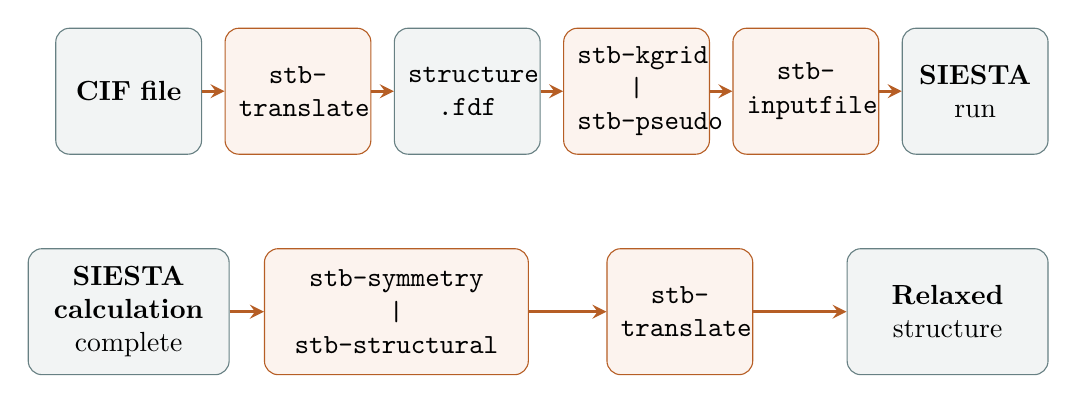
\begin{tikzpicture}[
		stage/.style={
			draw=stbteal!70,fill=stbteal!6,rounded corners=5pt,
			text width=1.5cm,minimum height=1.6cm,align=center,inner sep=5pt
		},
		tool/.style={
			stage,draw=stborange!85!black,fill=stborange!8
		},
		wide/.style={stage,text width=2.2cm},
		toolwide/.style={tool,text width=3cm},
		flow/.style={->,>=stealth,line width=1.2pt,draw=stborange!85!black}
	]
		\node[stage] (cif) at (0,1.4) {\textbf{CIF file}};
		\node[tool] (translate) at (2.15,1.4) {\texttt{stb-}\\\texttt{translate}};
		\node[stage] (structure) at (4.3,1.4) {\texttt{structure}\\\texttt{.fdf}};
		\node[tool] (tools) at (6.45,1.4) {
			\texttt{stb-kgrid}\\
			\texttt{|}\\
			\texttt{stb-pseudo}
		};
		\node[tool] (input) at (8.6,1.4) {\texttt{stb-}\\\texttt{inputfile}};
		\node[stage] (siesta) at (10.75,1.4) {\textbf{SIESTA}\\run};
		\draw[flow] (cif.east) -- (translate.west);
		\draw[flow] (translate.east) -- (structure.west);
		\draw[flow] (structure.east) -- (tools.west);
		\draw[flow] (tools.east) -- (input.west);
		\draw[flow] (input.east) -- (siesta.west);

		\node[wide] (complete) at (0,-1.4) {\textbf{SIESTA calculation}\\complete};
		\node[toolwide] (relax-tools) at (3.4,-1.4) {
			\texttt{stb-symmetry}\\
			\texttt{|}\\
			\texttt{stb-structural}
		};
		\node[tool] (relax-translate) at (7,-1.4) {\texttt{stb-}\\\texttt{translate}};
		\node[wide] (relaxed) at (10.4,-1.4) {\textbf{Relaxed}\\structure};
		\draw[flow] (complete.east) -- (relax-tools.west);
		\draw[flow] (relax-tools.east) -- (relax-translate.west);
		\draw[flow] (relax-translate.east) -- (relaxed.west);
	\end{tikzpicture}%
	}
	\vfill
\end{frame}

\section{Convergence Tests}

\begin{frame}{Three Numerical Dials, Three Directions}
	\centering
	{\large\bfseries Sweep the approximations before trusting the physics.}
	\par\vspace{0.35cm}
	\resizebox{0.96\textwidth}{!}{%
	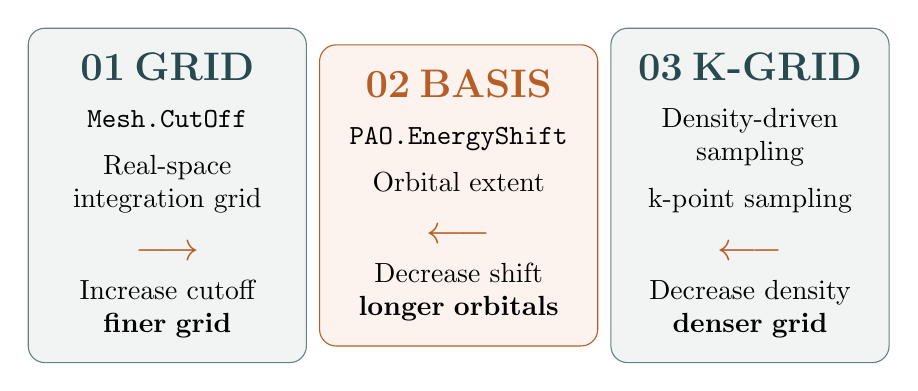
\begin{tikzpicture}[
		dial/.style={
			draw=stbteal!70,fill=stbteal!6,rounded corners=6pt,
			text width=2.9cm,minimum height=2.7cm,align=center,inner sep=9pt
		}
	]
		\node[dial] at (0,0) {
			{\color{stbteal}\Large\bfseries 01 GRID}\\[5pt]
			\texttt{Mesh.CutOff}\\[5pt]
			Real-space\\integration grid\\[7pt]
			{\color{stborange!85!black}\Large$\longrightarrow$}\\[2pt]
			Increase cutoff\\
			\textbf{finer grid}
		};
		\node[dial,draw=stborange!85!black,fill=stborange!8] at (3.7,0) {
			{\color{stborange!85!black}\Large\bfseries 02 BASIS}\\[5pt]
			\texttt{PAO.EnergyShift}\\[5pt]
			Orbital extent\\[7pt]
			{\color{stborange!85!black}\Large$\longleftarrow$}\\[2pt]
			Decrease shift\\
			\textbf{longer orbitals}
		};
		\node[dial] at (7.4,0) {
			{\color{stbteal}\Large\bfseries 03 K-GRID}\\[5pt]
			Density-driven sampling\\[5pt]
			k-point sampling\\[7pt]
			{\color{stborange!85!black}\Large$\longleftarrow$}\\[2pt]
			Decrease density\\
			\textbf{denser grid}
		};
	\end{tikzpicture}%
	}
	\vspace{0.25cm}
	\begin{alertblock}{The sweeps are independent}
		Converge k-grid first for metals or small gaps; then recheck mesh and basis
		using that denser sampling.
	\end{alertblock}
	\hfill{\scriptsize STB Manual, Section 11.5}
\end{frame}

\begin{frame}{Stage 1: Sweep, Relax, Run}
	\centering
	{\large\bfseries \texttt{stb-convergence} prepares the test; you run SIESTA.}
	\par\vspace{0.25cm}
	\resizebox{0.97\textwidth}{!}{%
	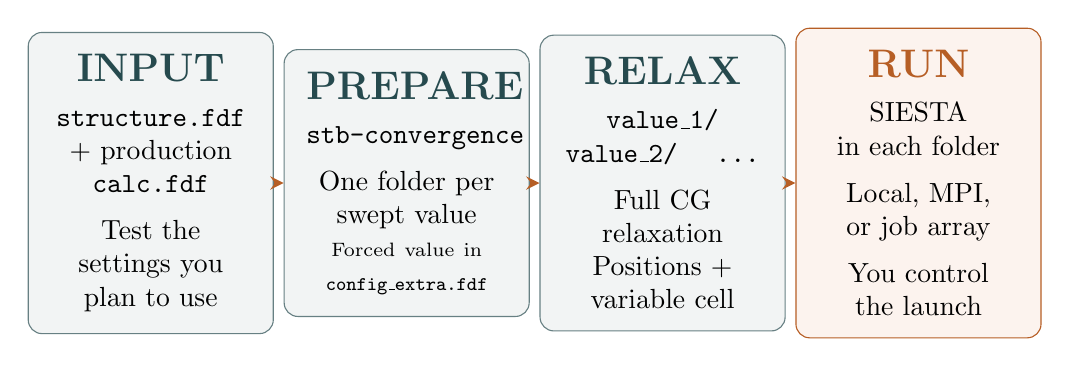
\begin{tikzpicture}[
		stage/.style={
			draw=stbteal!70,fill=stbteal!6,rounded corners=5pt,
			text width=2.55cm,minimum height=2.35cm,align=center,inner sep=8pt
		},
		run/.style={stage,draw=stborange!85!black,fill=stborange!8},
		flow/.style={->,>=stealth,line width=1.1pt,draw=stborange!85!black}
	]
		\node[stage] (input) at (0,0) {
			{\color{stbteal}\Large\bfseries INPUT}\\[4pt]
			\texttt{structure.fdf}\\
			+ production \texttt{calc.fdf}\\[5pt]
			Test the settings you plan to use
		};
		\node[stage] (prepare) at (3.25,0) {
			{\color{stbteal}\Large\bfseries PREPARE}\\[4pt]
			\texttt{stb-convergence}\\[5pt]
			One folder per swept value\\
			\scriptsize Forced value in \texttt{config\_extra.fdf}
		};
		\node[stage] (folders) at (6.5,0) {
			{\color{stbteal}\Large\bfseries RELAX}\\[4pt]
			\texttt{value\_1/ \quad value\_2/ \quad ...}\\[5pt]
			Full CG relaxation\\
			Positions + variable cell
		};
		\node[run] (siesta) at (9.75,0) {
			{\color{stborange!85!black}\Large\bfseries RUN}\\[4pt]
			SIESTA\\in each folder\\[5pt]
			Local, MPI, or job array\\[5pt]
			You control the launch
		};
		\draw[flow] (input.east) -- (prepare.west);
		\draw[flow] (prepare.east) -- (folders.west);
		\draw[flow] (folders.east) -- (siesta.west);
	\end{tikzpicture}%
	}
	\vspace{0.2cm}
	\begin{columns}[T]
		\begin{column}{0.40\textwidth}
			\metroset{block=fill}
			\begin{block}{Why relax every point?}
				The finite real-space grid creates an ``eggbox'' effect.
				At fixed geometry, energy may look settled while the relaxed
				cell is still drifting.
			\end{block}
		\end{column}
		\begin{column}{0.53\textwidth}
			\centering
			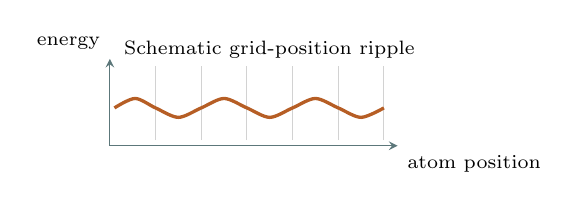
\begin{tikzpicture}[x=0.58cm,y=0.48cm]
				\foreach \x in {0,...,6} {
					\draw[gray!35] (\x,0.15)--(\x,2.1);
				}
				\draw[->,>=stealth,draw=stbteal!75] (0,0)--(6.3,0)
					node[below right,font=\scriptsize] {atom position};
				\draw[->,>=stealth,draw=stbteal!75] (0,0)--(0,2.3)
					node[above left,font=\scriptsize] {energy};
				\draw[stborange!85!black,line width=1.2pt]
					plot[smooth] coordinates {
						(0.1,1.0)(0.55,1.25)(1.0,1.0)(1.5,0.75)
						(2.0,1.0)(2.5,1.25)(3.0,1.0)(3.5,0.75)
						(4.0,1.0)(4.5,1.25)(5.0,1.0)(5.5,0.75)(6.0,1.0)
					};
				\node[font=\scriptsize,anchor=south west] at (0.1,2.05)
					{Schematic grid-position ripple};
			\end{tikzpicture}
		\end{column}
	\end{columns}
	\par\vspace{0.05cm}
	{\scriptsize STB Manual, Section 11.5}
\end{frame}

\begin{frame}{Stage 2: Two Plateaus, One Recommendation}
	\centering
	{\large\bfseries Energy and relaxed geometry must both converge.}
	\par\vspace{0.2cm}
	\begin{columns}[T]
		\begin{column}{0.49\textwidth}
			\metroset{block=fill}
			\begin{block}{Energy change}
				\centering
				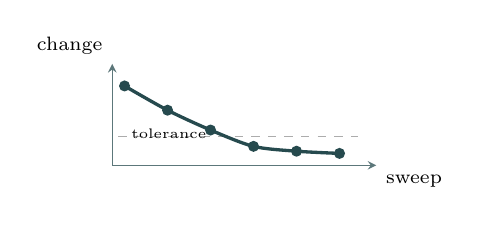
\begin{tikzpicture}[x=0.78cm,y=0.56cm]
					\draw[->,>=stealth,draw=stbteal!75] (0,0)--(4.3,0)
						node[below right,font=\scriptsize] {sweep};
					\draw[->,>=stealth,draw=stbteal!75] (0,0)--(0,2.3)
						node[above left,font=\scriptsize] {change};
					\draw[gray!65,dashed] (0.1,0.65)--(4.0,0.65);
					\node[font=\tiny,anchor=west] at (0.15,0.72) {tolerance};
					\draw[stbteal,line width=1.2pt]
						plot[smooth] coordinates {
							(0.2,1.8)(0.9,1.25)(1.6,0.8)(2.3,0.43)
							(3.0,0.32)(3.7,0.27)
						};
					\foreach \x/\y in {0.2/1.8,0.9/1.25,1.6/0.8,2.3/0.43,3.0/0.32,3.7/0.27}
						\fill[stbteal] (\x,\y) circle (2pt);
				\end{tikzpicture}
				{\scriptsize Default tolerance: $0.01$ eV/atom}
			\end{block}
		\end{column}
		\begin{column}{0.49\textwidth}
			\metroset{block=fill}
			\begin{block}{Relaxed-cell change}
				\centering
				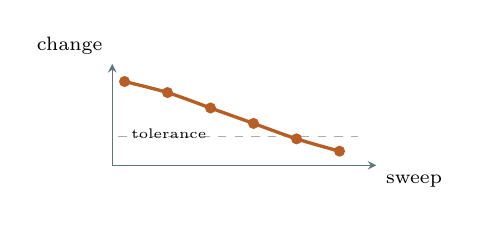
\begin{tikzpicture}[x=0.78cm,y=0.56cm]
					\draw[->,>=stealth,draw=stbteal!75] (0,0)--(4.3,0)
						node[below right,font=\scriptsize] {sweep};
					\draw[->,>=stealth,draw=stbteal!75] (0,0)--(0,2.3)
						node[above left,font=\scriptsize] {change};
					\draw[gray!65,dashed] (0.1,0.65)--(4.0,0.65);
					\node[font=\tiny,anchor=west] at (0.15,0.72) {tolerance};
					\draw[stborange!85!black,line width=1.2pt]
						plot[smooth] coordinates {
							(0.2,1.9)(0.9,1.65)(1.6,1.3)(2.3,0.95)
							(3.0,0.6)(3.7,0.32)
						};
					\foreach \x/\y in {0.2/1.9,0.9/1.65,1.6/1.3,2.3/0.95,3.0/0.6,3.7/0.32}
						\fill[stborange!85!black] (\x,\y) circle (2pt);
				\end{tikzpicture}
				{\scriptsize Default tolerance: $0.5\%$ in volume}
			\end{block}
		\end{column}
	\end{columns}
	{\scriptsize Schematic trends; each plot has its own scale.}
	\begin{alertblock}{Do not stop at the first flat-looking energy}
		Choose the more accurate value where both tests pass; the full remaining tail
		must stay within tolerance and SCF must be confirmed.
	\end{alertblock}
	{\scriptsize Quality flags are advisory, not plateau criteria.\\
	Optional \texttt{--apply} writes the recommendation to \texttt{calc.fdf}.\\
	STB Manual, Section 11.5}
\end{frame}

\section{Cohesive Energy}

\begin{frame}{Cohesive Energy: Binding in a Solid}
	\begin{columns}[T]
		\begin{column}{0.43\textwidth}
			\metroset{block=fill}
			\begin{block}{From free atoms to a crystal}
				\centering
				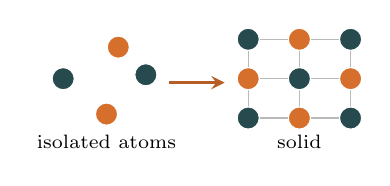
\begin{tikzpicture}[
					atomA/.style={circle,fill=stbteal,draw=white,minimum size=8pt,inner sep=0pt},
					atomB/.style={circle,fill=stborange,draw=white,minimum size=8pt,inner sep=0pt},
					flow/.style={->,>=stealth,line width=1.1pt,draw=stborange!85!black}
				]
					\node[atomA] at (0,0.55) {};
					\node[atomB] at (0.55,0.1) {};
					\node[atomA] at (1.05,0.6) {};
					\node[atomB] at (0.7,0.95) {};
					\node[font=\scriptsize] at (0.55,-0.25) {isolated atoms};
					\draw[flow] (1.35,0.5)--(2.05,0.5);
					\draw[gray!55] (2.35,0.05)--(3.65,0.05)--(3.65,1.05)--(2.35,1.05)--cycle;
					\draw[gray!55] (3.0,0.05)--(3.0,1.05);
					\draw[gray!55] (2.35,0.55)--(3.65,0.55);
					\node[atomA] at (2.35,0.05) {};
					\node[atomB] at (3.0,0.05) {};
					\node[atomA] at (3.65,0.05) {};
					\node[atomB] at (2.35,0.55) {};
					\node[atomA] at (3.0,0.55) {};
					\node[atomB] at (3.65,0.55) {};
					\node[atomA] at (2.35,1.05) {};
					\node[atomB] at (3.0,1.05) {};
					\node[atomA] at (3.65,1.05) {};
					\node[font=\scriptsize] at (3.0,-0.25) {solid};
				\end{tikzpicture}
			\end{block}
		\end{column}
		\begin{column}{0.55\textwidth}
			\metroset{block=fill}
			\begin{block}{Per-atom definition}
				\centering
				\[
					E_{\mathrm{coh}}=
					\frac{E_{\mathrm{bulk}}-\sum_{i=1}^{N}E_{\mathrm{atom}}(s_i)}{N}
				\]
			\end{block}
			\begin{itemize}
				\item Crystal energy vs. the same atoms isolated.
				\item $E_{\mathrm{coh}}<0$: bound; more negative means stronger binding.
				\item $-E_{\mathrm{coh}}$: energy per atom to separate the solid.
				\item Same basis and settings for bulk and atomic references.
			\end{itemize}
		\end{column}
	\end{columns}
	\vfill
	\hfill{\scriptsize STB Manual, Section 11.3}
\end{frame}

\begin{frame}{BSSE and Counterpoise: The Ghost-Atom Fix}
	\begin{columns}[T]
		\begin{column}{0.49\textwidth}
			\metroset{block=fill}
			\begin{block}{Why localized bases overbind}
				\centering
				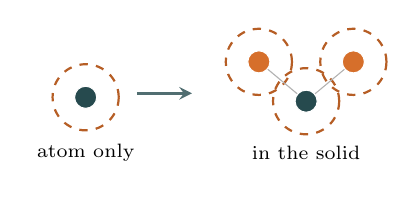
\begin{tikzpicture}[
					real/.style={circle,fill=stbteal,draw=white,minimum size=8pt,inner sep=0pt},
					neighbor/.style={circle,fill=stborange,draw=white,minimum size=8pt,inner sep=0pt},
					basis/.style={draw=stborange!85!black,dashed,line width=0.8pt},
					flow/.style={->,>=stealth,line width=1pt,draw=stbteal!80}
				]
					\draw[basis] (0,0) circle[radius=0.42];
					\node[real] at (0,0) {};
					\node[font=\scriptsize] at (0,-0.7) {atom only};
					\draw[flow] (0.65,0.05)--(1.35,0.05);
					\draw[basis] (2.2,0.45) circle[radius=0.42];
					\draw[basis] (2.8,-0.05) circle[radius=0.42];
					\draw[basis] (3.4,0.45) circle[radius=0.42];
					\draw[gray!60] (2.2,0.45)--(2.8,-0.05)--(3.4,0.45);
					\node[neighbor] at (2.2,0.45) {};
					\node[real] at (2.8,-0.05) {};
					\node[neighbor] at (3.4,0.45) {};
					\node[font=\scriptsize] at (2.8,-0.7) {in the solid};
				\end{tikzpicture}
				\begin{itemize}\footnotesize
					\setlength{\itemsep}{1pt}
					\item Localized LCAO/PAO basis functions.
					\item Neighbor orbitals lower the energy in the solid.
					\item Atomic reference too high $\Rightarrow$ $E_{\mathrm{coh}}$ too negative.
				\end{itemize}
			\end{block}
		\end{column}
		\begin{column}{0.49\textwidth}
			\metroset{block=fill}
			\begin{block}{Counterpoise: ghost neighbors}
				\centering
				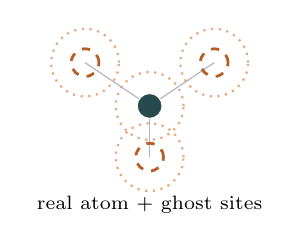
\begin{tikzpicture}[
					real/.style={circle,fill=stbteal,draw=white,minimum size=9pt,inner sep=0pt},
					ghost/.style={circle,draw=stborange!85!black,dashed,line width=1pt,minimum size=10pt,inner sep=0pt},
					basis/.style={draw=stborange!60,dotted,line width=0.8pt}
				]
					\draw[basis] (0,0) circle[radius=0.43];
					\draw[basis] (-0.82,0.55) circle[radius=0.43];
					\draw[basis] (0.82,0.55) circle[radius=0.43];
					\draw[basis] (0,-0.65) circle[radius=0.43];
					\draw[gray!60] (0,0)--(-0.82,0.55);
					\draw[gray!60] (0,0)--(0.82,0.55);
					\draw[gray!60] (0,0)--(0,-0.65);
					\node[real] at (0,0) {};
					\node[ghost] at (-0.82,0.55) {};
					\node[ghost] at (0.82,0.55) {};
					\node[ghost] at (0,-0.65) {};
					\node[font=\scriptsize] at (0,-1.25) {real atom + ghost sites};
				\end{tikzpicture}
				\begin{itemize}\footnotesize
					\setlength{\itemsep}{1pt}
					\item Ghosts add basis only: no nucleus or electrons.
					\item Recompute the atom with neighbors at crystal positions.
					\item \texttt{stb-cohesive} builds clusters; correction on by default.
				\end{itemize}
			\end{block}
		\end{column}
	\end{columns}
	\vspace{0.05cm}
	\metroset{block=fill}
	\begin{block}{Counterpoise-corrected cohesive energy}
		\centering
		\[
			E_{\mathrm{coh}}^{\mathrm{CP}}=
			\frac{E_{\mathrm{bulk}}-\sum_{i=1}^{N}E_{\mathrm{atom},i}^{\mathrm{ghost}}}{N}
		\]
		{\scriptsize STB Manual, Section 11.3}
	\end{block}
\end{frame}

	\begin{frame}{How STB Chooses Ghost Neighbors}
		\begin{columns}[T]
			\begin{column}{0.55\textwidth}
				\metroset{block=fill}
				\begin{block}{Neighbors within $R$ become ghosts}
					\centering
					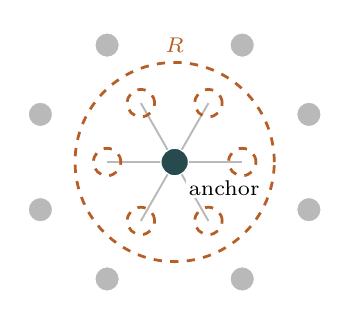
\begin{tikzpicture}[scale=1.1,transform shape,
						real/.style={circle,fill=stbteal,draw=white,minimum size=9pt,inner sep=0pt},
						ghost/.style={circle,draw=stborange!85!black,dashed,line width=1pt,minimum size=9pt,inner sep=0pt},
						excluded/.style={circle,fill=gray!55,draw=white,minimum size=8pt,inner sep=0pt},
						bond/.style={draw=gray!55,line width=0.7pt}
					]
						\draw[draw=stborange!85!black,dashed,line width=1pt] (0,0) circle[radius=1.15];
						\node[font=\scriptsize,text=stborange!85!black] at (0,1.35) {$R$};
						\foreach \x/\y in {0.78/0,0.39/0.68,-0.39/0.68,-0.78/0,-0.39/-0.68,0.39/-0.68} {
							\draw[bond] (0,0)--(\x,\y);
							\node[ghost] at (\x,\y) {};
						}
						\node[real] at (0,0) {};
						\node[font=\scriptsize,anchor=west,fill=white,inner sep=1pt] at (0.12,-0.3) {anchor};
						\foreach \x/\y in {1.55/0.55,0.78/1.35,-0.78/1.35,-1.55/0.55,-1.55/-0.55,-0.78/-1.35,0.78/-1.35,1.55/-0.55} {
							\node[excluded] at (\x,\y) {};
						}
					\end{tikzpicture}
					{\scriptsize Dashed: ghosts within $R$ \quad Gray: outside $R$}
				\end{block}
			\end{column}
			\begin{column}{0.41\textwidth}
				\metroset{block=fill}
				\begin{block}{Tune and verify}
					\centering
					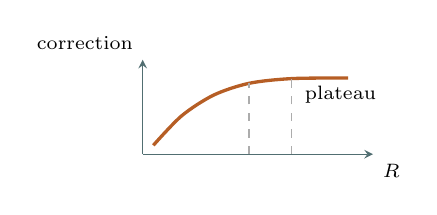
\begin{tikzpicture}[x=0.9cm,y=0.75cm]
						\draw[->,>=stealth,draw=stbteal!80] (0,0)--(3.25,0)
							node[below right,font=\scriptsize] {$R$};
						\draw[->,>=stealth,draw=stbteal!80] (0,0)--(0,1.6)
							node[above left,font=\scriptsize] {correction};
						\draw[stborange!85!black,line width=1.2pt]
							plot[smooth] coordinates {(0.15,0.15)(0.55,0.65)(1.0,1.0)(1.5,1.2)(2.1,1.28)(2.9,1.29)};
						\draw[gray!65,dashed] (1.5,0)--(1.5,1.2);
						\draw[gray!65,dashed] (2.1,0)--(2.1,1.28);
						\node[font=\scriptsize,anchor=west] at (2.15,1.0) {plateau};
					\end{tikzpicture}
					\begin{itemize}\footnotesize
						\setlength{\itemsep}{1pt}
						\item \texttt{--bsse-cutoff} $R$: default $4.0$ \AA.
						\item Shell count depends on bond length.
						\item Check \texttt{Ghost nb.}; zero means none included.
						\item \texttt{--bsse-convergence-check}: increase $R$; seek a plateau.
					\end{itemize}
				\end{block}
			\end{column}
		\end{columns}
		\vfill
		\hfill{\scriptsize STB Manual, Section 11.3}
	\end{frame}

	\begin{frame}{Symmetry Analysis}
		\begin{columns}[T]
			\begin{column}{0.95\textwidth}
				\metroset{block=fill}
				\begin{block}{Symmetry separates local environments}
					\centering
					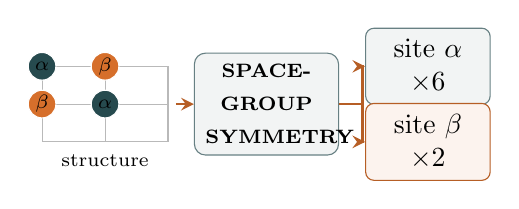
\begin{tikzpicture}[
						siteA/.style={circle,fill=stbteal,draw=white,minimum size=10pt,inner sep=0pt},
						siteB/.style={circle,fill=stborange,draw=white,minimum size=10pt,inner sep=0pt},
						sym/.style={draw=stbteal!70,fill=stbteal!6,rounded corners=4pt,text width=1.55cm,minimum height=0.8cm,align=center,inner sep=4pt},
						classA/.style={draw=stbteal!70,fill=stbteal!6,rounded corners=3pt,text width=1.3cm,align=center,inner sep=4pt},
						classB/.style={draw=stborange!85!black,fill=stborange!8,rounded corners=3pt,text width=1.3cm,align=center,inner sep=4pt},
						flow/.style={->,>=stealth,line width=1pt,draw=stborange!85!black}
					]
						\draw[gray!55] (-0.35,-0.48) rectangle (1.25,0.48);
						\draw[gray!55] (0.45,-0.48)--(0.45,0.48);
						\draw[gray!55] (-0.35,0)--(1.25,0);
						\node[siteA] at (-0.35,0.48) {\scriptsize$\alpha$};
						\node[siteB] at (0.45,0.48) {\scriptsize$\beta$};
						\node[siteB] at (-0.35,0) {\scriptsize$\beta$};
						\node[siteA] at (0.45,0) {\scriptsize$\alpha$};
						\node[font=\scriptsize] at (0.45,-0.72) {structure};
						\node[sym] (symmetry) at (2.5,0) {{\scriptsize\bfseries SPACE-GROUP}\\{\scriptsize\bfseries SYMMETRY}};
						\node[classA] (alpha) at (4.55,0.48) {site $\alpha$\\$\times 6$};
						\node[classB] (beta) at (4.55,-0.48) {site $\beta$\\$\times 2$};
						\draw[flow] (1.35,0)--(symmetry.west);
						\draw[flow] (symmetry.east)--++(0.3,0)|-(alpha.west);
						\draw[flow] (symmetry.east)--++(0.3,0)|-(beta.west);
					\end{tikzpicture}
					\[
						E_{\mathrm{ref}}=\frac{6E_{\alpha}+2E_{\beta}}{8}
					\]
					\begin{itemize}\footnotesize
						\setlength{\itemsep}{1pt}
						\item One ghost cluster per inequivalent site.
						\item Weight references by site multiplicity, not a flat average.
					\end{itemize}
				\end{block}
			\end{column}
		\end{columns}
		\vfill
		\hfill{\scriptsize STB Manual, Section 11.3}
	\end{frame}

	\begin{frame}{stb-cohesive: End-to-End Workflow}
		\centering
		\vspace{0.2cm}
		\resizebox{0.98\textwidth}{!}{%
		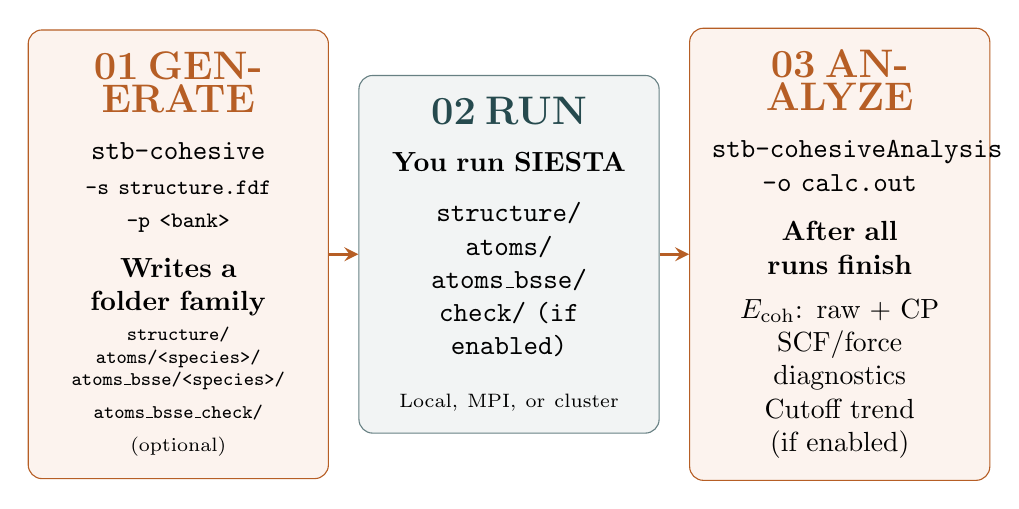
\begin{tikzpicture}[
			stage/.style={
				draw=stbteal!70,fill=stbteal!6,rounded corners=5pt,
				text width=3.25cm,minimum height=4.3cm,align=center,inner sep=8pt
			},
			tool/.style={stage,draw=stborange!85!black,fill=stborange!8},
			flow/.style={->,>=stealth,line width=1.2pt,draw=stborange!85!black}
		]
			\node[tool] (generate) at (0,0) {
				{\color{stborange!85!black}\Large\bfseries 01 GENERATE}\\[5pt]
				\texttt{stb-cohesive}\\[3pt]
				{\footnotesize\texttt{-s structure.fdf}\\\texttt{-p <bank>}}\\[6pt]
				\textbf{Writes a folder family}\\[3pt]
				{\scriptsize
				\texttt{structure/}\\
				\texttt{atoms/<species>/}\\
				\texttt{atoms\_bsse/<species>/}\\
				\texttt{atoms\_bsse\_check/} (optional)}
			};
			\node[stage] (run) at (4.2,0) {
				{\color{stbteal}\Large\bfseries 02 RUN}\\[5pt]
				\textbf{You run SIESTA}\\[6pt]
				\texttt{structure/}\\
				\texttt{atoms/}\\
				\texttt{atoms\_bsse/}\\
				\texttt{check/ (if enabled)}\\[7pt]
				{\scriptsize Local, MPI, or cluster}
			};
			\node[tool] (analyze) at (8.4,0) {
				{\color{stborange!85!black}\Large\bfseries 03 ANALYZE}\\[5pt]
				\texttt{stb-cohesiveAnalysis}\\
				\texttt{-o calc.out}\\[6pt]
				\textbf{After all runs finish}\\[4pt]
				$E_{\mathrm{coh}}$: raw + CP\\
				SCF/force diagnostics\\
				Cutoff trend (if enabled)
			};
			\draw[flow] (generate.east) -- (run.west);
			\draw[flow] (run.east) -- (analyze.west);
		\end{tikzpicture}%
		}
		\vspace{0.25cm}
		\begin{alertblock}{Key handoff}
			Stage 1 prepares folders; it does not launch SIESTA. Run every generated folder before analysis.
		\end{alertblock}
		\hfill{\scriptsize STB Manual, Section 11.3}
	\end{frame}

	\section{Next ...}

\begin{frame}{Acknowledgments}
	\begin{center}
		\large
		First, I would like to thank the \textbf{SEEDMOL COMMITE},
		for the invitation.

		\vspace{0.6cm}

		I gratefully acknowledge the funding agencies.
		I also thank the national HPC centers \textbf{Santos Dumont/LNCC} and \textbf{CENAPAD}.

		\vspace{0.5cm}

		\begin{columns}[c]
			\column{0.25\textwidth}
			
\includegraphics[width=\linewidth]{figures/cnpq.png}
			\column{0.25\textwidth}
			
\includegraphics[width=\linewidth]{figures/fapdf.png}
			\column{0.25\textwidth}
			
\includegraphics[width=\linewidth]{figures/capes.jpg}
		\end{columns}
	\end{center}
\end{frame}

\begin{frame}{University of Brasilia}
	Laboratório de Computação em Ciência de Materiais (LCCMat)
	\vspace{1cm}
	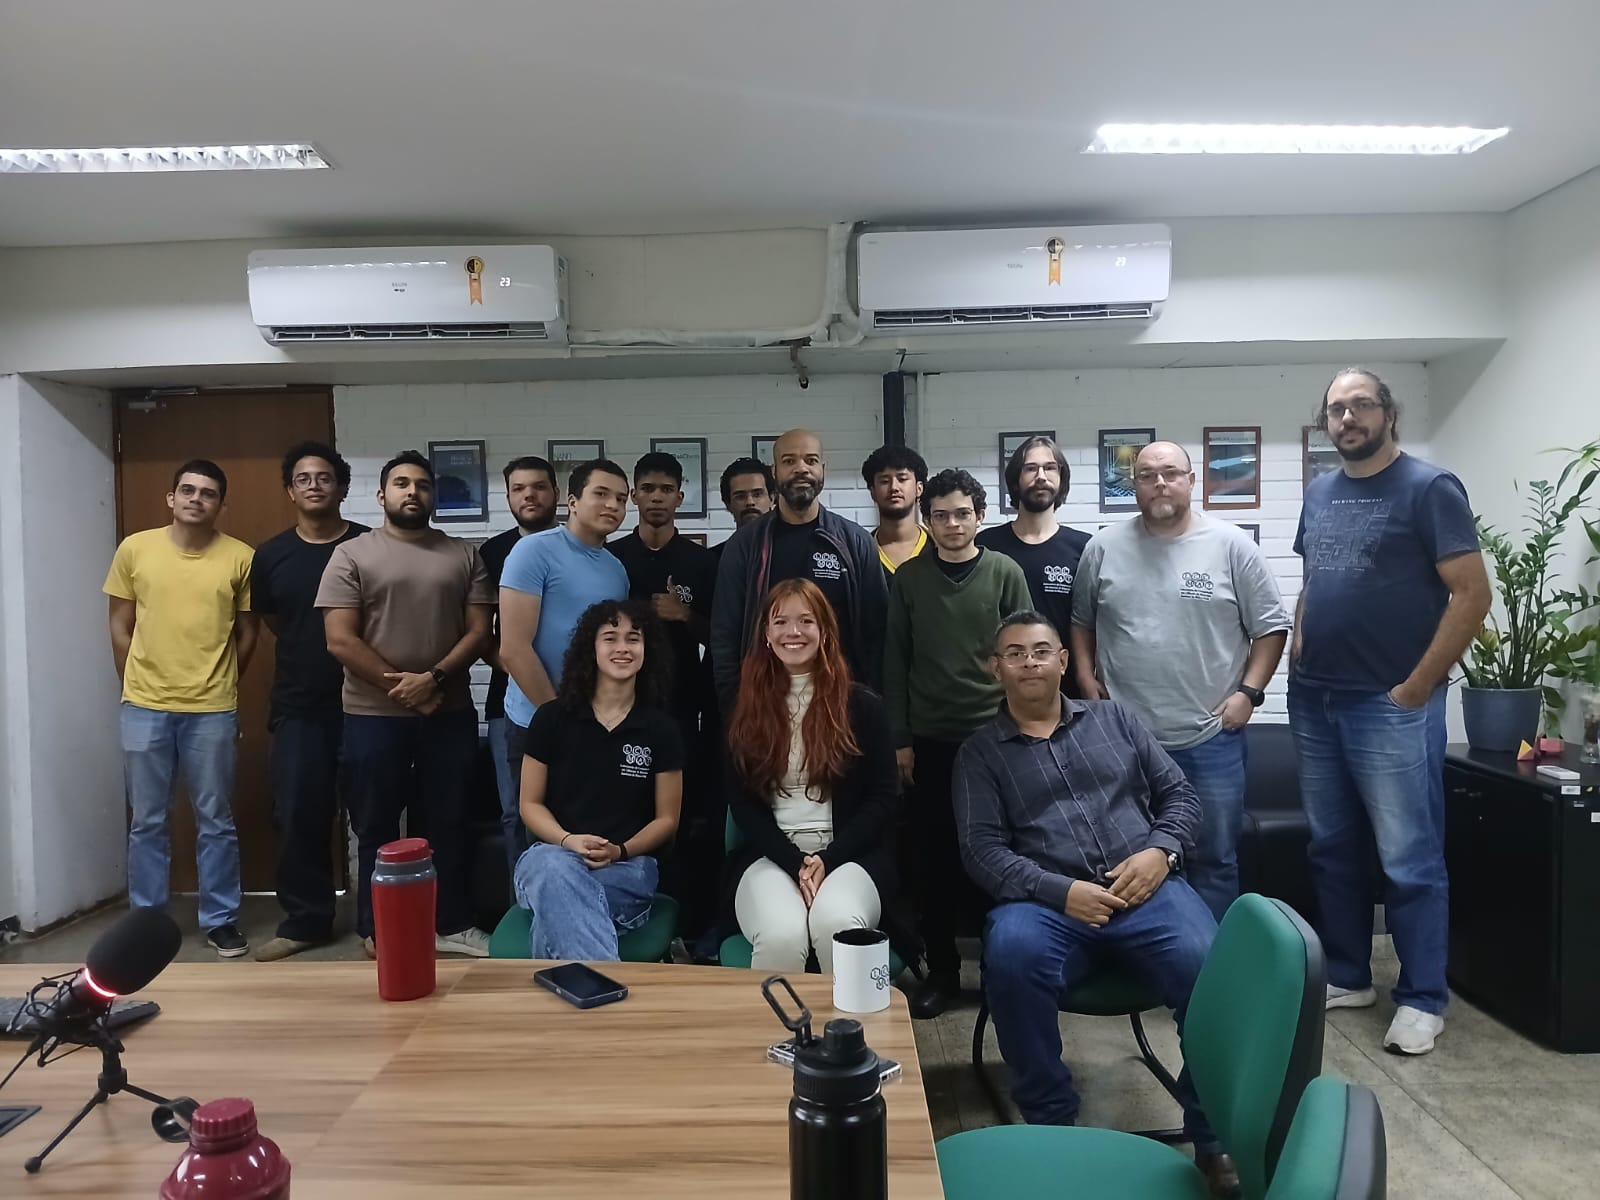
\includegraphics[width=\textwidth]{figures/lccmat.jpeg}
\end{frame}

% --- CONTACT & THANK YOU SLIDE ---
\begin{frame}
\frametitle{Thank You \& Let's Connect!}
\begin{columns}[c] % 'c' for vertically centered columns

    \column{0.4\textwidth}
        \centering
        % This QR code will generate a mailto link
        \qrcode[height=4cm]{https://bastoscmo.github.io/}
        \vspace{0.5cm}

        \large{my email: carlos.bastos@unb.br}

    \column{0.6\textwidth}
        \large
        We're always open to new collaborations...

        \vspace{0.7cm}

        ...especially if they involve discussing physics over a good cup of coffee!

	
\includegraphics[height=3cm]{figures/cofee.png}

        \vspace{1cm}

        \huge{\textbf{Thank you!}}

\end{columns}
\end{frame}

\end{document}
